\documentclass[a4paper, twoside, 12pt, french]{report}

\usepackage[utf8]{inputenc}
\usepackage[T1]{fontenc}
\usepackage[francais]{babel}
\usepackage{lmodern}
\usepackage[top=3cm, bottom=3cm, left=3cm, right=3cm]{geometry}
\usepackage{graphicx}
\usepackage{cite}
\usepackage[nottoc,notlot,notlof]{tocbibind} % Ajoute la bibliographie dans la table des matières (toc)
\usepackage{setspace} % Interligne
\usepackage{fancyhdr} % Hauts de page
\usepackage{hyperref} % Liens
\usepackage{listings} % Code
\usepackage{multicol} % Colonnes

%%%%% Header %%%%%
\fancyhead[RO,LE]{\thepage}
\fancyhead[LO]{\itshape\nouppercase{\leftmark}}
\fancyhead[RE]{\itshape\nouppercase{\rightmark}}
\fancyfoot{}

%\renewcommand{\headrulewidth}{0pt} % Epaisseur de la ligne sous le header
\geometry{headheight=16pt} % Nécessaire pour fancyhdr
%\setlength{\headheight}{16pt} % Nécessaire pour fancyhdr

\raggedbottom % Evite que la page couvre tout l'espace vertical avec des espaces

%%%%% Code %%%%%
\lstset{
	breaklines=true,
	numbers=left,
	numbersep=10pt,
	basicstyle=\fontsize{11}{12}\selectfont\ttfamily,
	frame=lrtb
}
\lstdefinestyle{dig}{
	breaklines=true,
	basicstyle=\fontsize{10}{9}\selectfont\ttfamily,
	frame=lrtb
}

\onehalfspacing

\begin{document}

\newgeometry{top=2.5cm, bottom=2.5cm, left=2.5cm, right=2.5cm}
\begin{titlepage}
\center

\textsc{\LARGE Université catholique de Louvain}\\[1cm]
\textsc{\Large Travail de fin d'études}\\[2cm]


\includegraphics[scale=.15]{UCL_mention_pantone282.jpg}\\[1.5cm]

% Titre
\textsc{\Large Analyse du traçage des utilisateurs\\via leur navigateur Web}\\[1.5cm]

\begin{minipage}{0.4\textwidth}
\begin{center}
%\large \emph{Auteur :} \\
\large Antoine \textsc{Marchal}
\end{center}
\end{minipage}\\[2cm]

\begin{minipage}{0.4\textwidth}
\begin{flushleft} \large
\emph{Promoteur :} \\
Olivier \textsc{Bonaventure}\\
\emph{Co-promoteur :} \\
Pierre \textsc{Reinbold}\\
\emph{Lecteur :} \\
\textsc{Xavier Carpent}
\end{flushleft}
\end{minipage}
~
\begin{minipage}{0.5\textwidth}
\begin{flushright} \large
{\normalsize Mémoire présenté en vue de\\
l'obtention du grade de\\
\emph{Master [120] en Sciences Informatiques}\\
(option \emph{sécurité \& réseaux informatiques})}
\end{flushright}
\end{minipage}\\[1.5cm]


{\huge Version temporaire, compilée le \today}
%{\normalsize Louvain-la-Neuve, Belgique}\\
%{\normalsize Année académique 2013-2014}

\end{titlepage}
\restoregeometry

%%% Table des matières
\pagenumbering{arabic} % Remise à 1
\addtocontents{toc}{\protect\thispagestyle{empty}} % Enlève le numéro de page sur la première page du toc
\pagestyle{empty} % Enlève le numéro de page sur les autres pages du toc
%\newgeometry{top=1.5cm, bottom=2cm, left=2.5cm, right=2.5cm}
\tableofcontents
\restoregeometry
\clearpage % Nécessaire pour ne pas avoir fancyhdr sur la dernière page du toc
%%%
\pagestyle{fancy}
\chapter{Introduction}
\section{Motivation et problématique}
Notre navigation sur Internet est de plus en plus scrutée par diverses organisations, que ce soient des entreprises commerciales ou des agences gouvernementales. D'ailleurs, des révélations récentes d'Edward Snowden \cite{WikipediaFR_RES}, un informaticien américain et ancien employé de la CIA et de la NSA, ont permis de mettre en lumière un système élaboré destiné à surveiller les utilisateurs d'Internet.

Ce travail se focalise sur la surveillance opérée par les entreprises commerciales. En effet, elles essaient de nous suivre à la trace afin de déterminer nos habitudes et nos préférences. Avec l'aide de ces précieuses informations, elles peuvent alors mieux cibler nos besoins et nous proposer des biens et des services qui sont censés nous intéresser davantage, voire anticiper nos intentions\cite{MD1}.

Cette pratique est de plus en plus répandue sur les sites de vente en ligne, grâce à l'historique de nos consultations et achats.

D'autres formes de surveillance plus vicieuses existent également. Imaginons que vous souhaitiez voyager vers un pays exotique et que vous consultez le prix des billets d'avion vers cette destination sur le site d'une compagnie aérienne. Lors d'une consultation ultérieure, le prix a augmenté et vous vous empressez alors d'acheter le billet craignant que son prix ne continue d'augmenter. Malheureusement pour vous, celui-ci a en fait été gonflé pour vous pousser à l'achat.

Les plus grosses régies publicitaires sont installées sur un grand nombre de sites et lors de chaque visite, elles enregistrent les traces que vous laissez. En regroupant toutes les informations disséminées sur ces différents sites, elles sont alors en mesure d'établir votre profil. Les détails de celui-ci peuvent se revendre à prix d'or auprès d'autres compagnies. Il est évidemment plus facile de cibler un segment constitué de personnes dont on connaît le profil sociodémographique, le sexe, l'âge, les intérêts,...

Avez-vous déjà remarqué que le contenu des publicités s'adaptait en fonction de vos requêtes effectuées sur les moteurs de recherche ou des sites que vous visitez ?

Comme vous pouvez le remarquer avec ces différents exemples de la vie quotidienne, la surveillance des utilisateurs d'Internet peut générer plusieurs inconvénients qui nous touchent directement. Il est donc intéressant d'analyser cette surveillance et déterminer par quels moyens elle s'opère. Afin de préserver notre vie privée sur Internet, il est nécessaire de connaître comment nous sommes identifiés. Il faut également s'assurer que les outils dont nous disposons afin de nous protéger soient réellement efficaces et adaptés à nos besoins.


%%%%%%%%%%%%%%%%%%%%%%%%%%%%%%
\section{La vie privée}
Le respect de la vie privée est intimement lié à l'évolution de la surveillance.
Il y a toujours eu des conflits entre les personnes qui estiment que tout le monde doit pouvoir utiliser et partager une technologie permettant de sécuriser ses communications et les gouvernements qui souhaiteraient garder la possibilité d'écouter ces communications. Prenons l'exemple du gouvernement américain qui avait peur de passer d'un monde où il avait un contrôle total à un monde où il n'en avait plus. En conséquence, il a considéré l'export de la cryptographie hors des USA équivalent à l'export de munitions. Ainsi, afin de dévoiler les sources de PGP (Pretty Good Privacy, un logiciel de chiffrement et de déchiffrement cryptographique) au monde entier, son auteur a usé d'une astuce en publiant un livre qui en contient le code source complet (l'export de livres est protégé par le Premier Amendement) \cite{youtube_moxie_marlinspike}.
\newline

Les programmes de surveillance du passé peuvent être considérés comme de la "surveillance de proximité", où un gouvernement tentait d'utiliser la technologie afin de surveiller les communications lui-même. Les programmes actuels marquent une transition vers la "surveillance oblique" dans laquelle un gouvernement va plus souvent se rendre aux endroits où les informations sont accumulées (fournisseurs d'adresses e-mail, moteurs de recherche, réseaux sociaux et télécoms) \cite{wired_nothing_to_hide}.
\newline

En 2001, John Poindexter, alors qu'il occupait un poste officiel au sein du Département de la Défense des Etats-Unis, a voulu mettre en place le programme \textit{Total Information Awareness} qui consistait en un système de data mining. Celui-ci devait enregistrer tous les e-mails, tout le trafic web, tout l'historique des cartes de crédit et tous les dossiers médicaux. Le but était ensuite de développer une technologie afin d'extraire les données dont on avait besoin. Lors de sa conférence à la DEF CON 18, Moxie Marlinspike \footnote{Moxie Marlinspike est le pseudonyme d'un chercheur en sécurité informatique qui est engagé dans le respect de la vie privée \cite{site_perso_moxie_marlinspike}.} a tourné en ridicule le logo du programme (\autoref{IAO_logo}) en expliquant qu'il était déconseillé d'utiliser un logo qui inspirait la peur. D'ailleurs, le projet a été annulé car il a reçu beaucoup de contestations. Cependant, lorsque l'on regarde ce que Google fait aujourd'hui, c'est exactement la même chose, voire pire. Or, personne ne proteste et de surcroît, tout le monde utilise ses services !
\begin{itemize}
  \item Les emails sont enregistrés par Gmail.
  \item Le trafic web est enregistré par Google Analytics.
  \item L'historique des cartes de crédit est enregistré par Google Checkout.
  \item Les dossiers médicaux sont enregistrés par Google Health.
  \item L'historique des positions GPS est enregistré par Android.
  \item ...
  %\newline
\end{itemize}
De plus, on sait que Google a la capacité d'extraire de manière efficace les informations qu'il désire afin de les monétiser avec des publicités. Lorsque le CEO de Google, Eric Schmidt, déclare : "If you have something that you don't want anyone to know, maybe you shouldn't be doing it in the first place" \cite{privacy_eric_schmidt}, cela fait froid dans le dos.

\begin{figure}[h]
	\centering
	
\includegraphics[scale=0.2]{figures/IAO-logo.png}
	\caption{\label{IAO_logo}Le logo officiel du programme \textit{Total Information Awareness}}.
\end{figure}

Dans sa conférence, Moxie Marlinspike utilise un autre exemple : personne n'accepterait de porter un trackeur monitoré par l'Etat mais tout le monde possède et porte un GSM en permanence. Or, celui-ci envoie en temps réel sa position à l'opérateur qui est obligé de délivrer cette information si on la lui demande. Pour lui, il y a cependant une différence essentielle : le choix. Nous choisissons de posséder un GSM afin de communiquer mais nous refuserions un dispositif de traçage s'il nous était imposé.
\newline

%%%%%

Maintenant, passons au sujet de la vie privée.\\
D'après Moglen \footnote{Eben Moglen est professeur de droit et d'histoire du droit à l'Université Columbia. Il est le président du Software Freedom Law Center, une organisation qui procure assistance et défense juridique aux développeurs de logiciels libres et open-source.} \cite{Moglen_part2}, le concept de vie privée englobe 3 éléments.
\begin{itemize}
  \item La confidentialité : la capacité de garder des messages privés c'est-à-dire que leur contenu n'est connu que de ceux à qui ils sont destinés.
  \item L'anonymat : la capacité d'envoyer des messages sans savoir de qui ils proviennent ni à qui ils sont destinés, même si leur contenu est ouvert.
  \item L'indépendance : la capacité de prendre des décisions librement, sans que la confidentialité ou l'anonymat ne soient violés.
\end{itemize}

Pour lui, si l'un de ces éléments n'est pas respecté, on ne peut pas avoir de gouvernement démocratique car la vie privée en est une condition nécessaire.
\newline

Il explique également qu'on ne devrait pas voir la vie privée comme une transaction. En effet, ceux qui veulent profiter de nos informations souhaitent définir la vie privée comme un concept que l'on peut négocier. Ainsi, ils nous offrent un service gratuit comme l'accès à une messagerie mais en échange, ils lisent nos mails. Pour eux, il s'agirait seulement d'une transaction entre deux parties. Cependant, si on y réfléchit, ce n'est pas une transaction quelconque car tous ceux qui nous écrivent sont aussi impliqués dans cet accord, qui était supposé être bilatéral.

Rien n'est gratuit dans la vie et cela l'est également sur Internet. En réalité, le prix à payer est de dévoiler des informations personnelles qui peuvent potentiellement être exploitées afin de rapporter de l'argent.
\newline

Les exemples de l'introduction montrent déjà clairement que la surveillance des sites web peut nous coûter de l'argent en nous incitant à consommer plus. Mais les risques de cette surveillance peuvent aller bien au-delà. En effet, la liste des sites web visités par une personne peut en révéler beaucoup sur sa situation familiale, financière ou sanitaire.
\newline

Imaginons une situation où le directeur des ressources humaines d'une entreprise reçoit des CV. Il décide de trouver davantage d'informations au sujet des candidats et pour cela, tape leur nom dans un moteur de recherche. Il pourrait tomber sur la photo d'une jeune femme portant un bébé dans ses bras ou sur la photo d'une jeune femme seule. Pensez-vous qu'elles aient la même chance d'être rappelées pour un entretien ?

Lors d'une expérience menée avec son équipe \cite{TED_Alessandro_Acquisti}, Alessandro Acquisti \footnote{Alessandro Acquisti est un économiste comportemental à l'Université Carnegie Mellon et il étudie l'économie comportementale de la vie privée.} a créé des profils Facebook en modifiant certaines de leurs caractéristiques. Il a ensuite envoyé des candidatures à différentes entreprises américaines et a analysé leur comportement face aux profils associés aux candidatures. Les résultats de l'expérience ont montré que les entreprises agissaient en fonction des informations qu'elles avaient trouvées sur les réseaux sociaux.
\newline

Face à la montée de la surveillance, certaines personnes émettent le désir de préserver leur vie privée. On leur rétorque souvent "Si vous ne faites rien de mal, qu'avez-vous à cacher ?".
D'après Bruce Schneier \footnote{Bruce Schneier est un cryptologue, spécialiste en sécurité informatique et écrivain américain.} \cite{the_eternal_value_of_privacy}, la vie privée n'a rien à voir avec le fait d'avoir quelque chose de négatif à cacher, c'est un besoin humain essentiel.
Nous faisons énormément de choses en privé qui ne sont pas considérées comme illégales mais que nous préférons garder pour nous. Mettre des rideaux à ses fenêtres n'est pas criminel, cela traduit juste notre envie de garder notre intimité, vie privée.
Ce qui l'ennuie c'est qu'on présuppose que la vie privée sert à dissumuler des mauvaises actions alors que ce n'est pas le cas. Il affirme même que le droit à une vie privée est un droit de l'être humain. D'ailleurs, lorsque la Constitution américaine fut rédigée, le principe de vie privée n'y a pas été inscrit car il était considéré comme inhérent aux êtres. A l'époque, on ne surveillait que les criminels, pas les honnêtes citoyens.

Lorsqu'une personne se sent surveillée, elle n'agit plus de la même façon. Cela vous est sûrement déjà arrivé de cesser votre conversation si vous sentiez que vous étiez observé par peur que vos mots ne soient sortis de leur contexte. Une surveillance généralisée a le même effet mais sur un ensemble de personnes beaucoup plus étendu.
\newline

Est-ce que les personnes déclarant ne rien avoir à cacher resteraient du même si leur gouvernement, avec l'aide de toutes les informations qu'il possède grâce à la surveillance, décidait que leurs actions étaient suspectes et que des sanctions étaient appliquées arbitrairement ?\\
Une simple question pourrait également les raisonner : donneriez-vous votre adresse, numéro de téléphone, numéro de carte de crédit et autres données personnelles à un inconnu dans la rue ?

%%%%%%%%%%%%%%%%%%%%%%%%%%%%%%
\section{Méthodologie utilisée}
Afin de répondre à la problématique de la surveillance sur Internet, il faut tout d'abord comprendre comment Internet fonctionne et en particulier, certains de ses mécanismes tels que les cookies.

Ensuite, il faut identifier la manière dont ces mécanismes peuvent être utilisés ou détournés afin de permettre le traçage des utilisateurs.

Grâce à ces connaissances, nous serons en mesure de détecter quels sont les moyens effectivement utilisés par les sites qui pratiquent cette surveillance et d'estimer son étendue sur un panel constitué des principaux sites web (classement Alexa \cite{AlexaTop}).

Pour terminer, nous pourrons déterminer si les outils censés protéger notre vie privée sont réellement efficaces. % et par quels moyens nous pourrions les améliorer.


\chapter{Protocoles et mécanismes d'Internet}

\section{Présentation du protocole HTTP}
HTTP (HyperText Transport Protocol) \cite{Obo_CNP3} est un protocole qui fournit les fondations du World Wide Web, il repose sur le modèle client-serveur dans lequel le client envoie une requête et le serveur retourne une réponse. Il est décrit par la RFC 2616 \cite{IETF_RFC2616}.

Les requêtes HTTP se composent de trois parties :
\begin{enumerate}
	\item Une ligne de requête (qui contient notamment une URI)
	\item Des entêtes (qui contiennent des paramètres pour la requête)
	\item Le corps de la requête (optionnel)
	\newline
\end{enumerate}

Lorsqu'un utilisateur clique sur un lien hypertexte via son navigateur, celui-ci se connecte à un serveur identifié par l'URI "Uniform Resource Identifier" présent dans ce lien. Le navigateur envoie alors une requête à laquelle le serveur répond puis le navigateur se déconnecte du serveur. On considère que la requête est sans état car à chaque fois que le navigateur crée une connexion pour une requête, le serveur la traite comme si c'était la première ; les requêtes sont donc indépendantes.

Les réponses HTTP se composent également de trois parties :
\begin{enumerate}
	\item Une ligne de statut (qui indique si la requête est réussie ou pas)
	\item Des entêtes (qui contiennent des informations sur la réponse)
	\item Le corps de la réponse
	\newline
\end{enumerate}

Il fallait trouver une solution afin d'avoir la possibilité de garder une certaine quantité d'informations entre des requêtes successives. En effet, si le serveur est dans l'incapacité de se souvenir de ce que le client a fait auparavant, il est par exemple impossible de développer un site de e-commerce étant donné que celui-ci ne sauvegarderait pas la liste des articles du panier virtuel.

Une première solution consistait à forcer l'authentification du client (comme pour FTP) mais ce n'est pas toujours nécessaire ou applicable sur tous les sites web.

Une seconde solution était d'utiliser les différents types d'entêtes \emph{Accept-*}. Par exemple, un client aurait pu utiliser l'entête \emph{Accept-Language} pour indiquer la langue dans laquelle il voulait visiter le site. Cependant, cela fournit des possibilités assez limitées car cet entête est réglé par le navigateur et l'utilisateur aurait été dans l'impossibilité d'indiquer une langue différente pour chaque site visité sans devoir effectuer une manipulation conséquente.

Une autre solution, qui est la plus largement adoptée, est l'utilisation d'un cookie HTTP. Elle est expliquée plus en détail dans la section suivante.
%\newline

Des exemples de requête et réponse HTTP sont disponibles dans la \autoref{http_request_example}.


%%%%%%%%%%%%%%%%%%%%%%%%%%%%%%
\section{Cookies}
Une première description informelle sur les cookies a été publiée sur le site web de Netscape Communications. Le processus de standardisation des cookies a commencé en avril 1995 sur la liste de diffusion [www-talk], ensuite, l'IETF (Internet Engineering Task Force) a entrepris d'écrire un standard pour les cookies \cite{Kristol:2001:HCS:502152.502153}. C'est ainsi que la première RFC (RFC 2109) sur les cookies est parue en février 1997 \cite{IETF_RFC2109}, rendue obsolète en octobre 2000 par la RFC 2965 \cite{IETF_RFC2965}. Elle a également été remplacée, par la RFC 6265 en avril 2011 \cite{IETF_RFC6265}, qui est toujours d'application en ce jour et constitue la référence en ce qui concerne les cookies. Il est intéressant de noter qu'une section dédiée à la vie privée (section 7) est présente dans cette dernière RFC, ce qui constitue une nouveauté.
\newline

Un cookie est un petit fichier stocké en clair sur le disque dur de l'utilisateur par le navigateur. Il fait le lien entre la session de l'utilisateur et les données enregistrées par le site web (dans une base de données par exemple). Les cookies sont transmis dans les entêtes des requêtes et des réponses HTTP \cite{IETF_RFC6265}.

Notez que certains navigateurs actuels enregistrent désormais ces cookies dans une base de données. C'est notamment le cas pour Firefox 3 qui enregistre ses cookies dans une base de données SQLite.
%\newline

Dans sa réponse à une requête, un serveur peut envoyer des informations arbitraires (le cookie) dans un entête \textit{Set-Cookie}. Le client a le choix d'ignorer cet entête. S'il l'accepte, l'information présente dans l'entête peut contenir n'importe quoi et c'est elle qui permet au serveur de continuer là où il en était. Il peut s'agir d'un identifiant relatif à l'utilisateur, une clé dans une base de données,...
Le serveur peut ajouter des attributs afin de configurer les cookies (sections 5.2.1 à 5.2.6 de la RFC 6265) \cite{IETF_RFC6265} :

\begin{itemize}
	\item Expires et Max-Age : date d'expiration
	\item Domain : domaine
	\item Path : chemin
	\item Secure et HttpOnly : type de connexion
	\newline
\end{itemize}

Grâce aux attributs \textit{Domain} et \textit{Path}, le serveur peut décider à qui le client va renvoyer cette information. Par exemple, avec un attribut \textit{Domain=exemple.com} et un attribut \textit{Path=/}, le serveur demande au client de renvoyer le cookie dans chaque requête vers tout sous-domaine et chemin de \textit{exemple.com}.
\newline

Lorsqu'une requête est envoyée à un serveur et si l'URI présente dans cette requête correspond aux attributs \textit{Domain} et \textit{Path} d'un cookie enregistré chez le client, celui-ci l'ajoute à sa requête.
Habituellement, le client est coopératif et renvoie l'information du cookie qui est stocké par le navigateur. Ainsi, dans chaque requête ultérieure qu'il fait vers le serveur, le client indique cette information dans un entête \textit{Cookie}. Le serveur peut choisir de renvoyer un nouveau cookie dans ses réponses, ce qui remplacera automatiquement l'ancien cookie. Il peut également supprimer un cookie en renvoyant un entête \textit{Set-Cookie} avec une date d'expiration dans le passé. Le cookie sera supprimé seulement si les attributs \textit{Path} et \textit{Domain} dans l'entête \textit{Set-Cookie} correspondent aux valeurs utilisées lorsque le cookie a été créé.
\newline

Il y a un contrat implicite entre le client et le serveur : le serveur compte sur le client pour lui retourner son état lors de la prochaine requête. Un cookie est donc une donnée que le serveur et le client se renvoient l'un à l'autre. La quantité d'informations est généralement petite et à la discrétion du serveur. En effet, la plupart du temps, analyser le contenu du cookie ne révèle ni à quoi il est destiné ni la valeur qu'il représente.


%%%%%%%%%%%%%%%%%%%%%%%%%%%%%%
\section{Cache}
Dans le domaine informatique, un cache permet de garder une copie locale d'un élément afin de répondre rapidement à une requête. Au lieu de récupérer l'élément, le cache renvoie sa copie, ce qui permet de réduire sensiblement le temps de réponse.\\
Le principe de cache sur le protocole HTTP est défini dans la RFC 2616 \cite{IETF_RFC2616} (sections 13 et 14). Les mécanismes de cache peuvent être implémentés à différents niveaux :
\begin{itemize}
  \item sur le réseau qui délivre le contenu d'un site web (ex. : un CDN - "Content Delivery Network")
  \item sur l'application qui gère et affiche le contenu d'un site web (ex. : un CMS - "Content Management System")
  \item sur le serveur qui héberge le site web (ex. : Apache)
  \item via le navigateur Web du client qui stocke les fichiers sur le disque dur
  \newline
\end{itemize}

Lorsqu'on navigue sur Internet, le cache du navigateur enregistre certaines ressources (images, feuilles de style, fichiers JavaScript, etc.) afin de ne pas devoir les recharger depuis le serveur lors des visites ultérieures. Par ailleurs, les administrateurs d'un site web peuvent paramétrer la mise en cache de certains éléments grâce à l'entête \textit{Cache-Control}. Celui-ci est utilisé pour spécifier des directives qui doivent être respectées par tous les mécanismes de cache le long de la chaîne requête-réponse. Grâce à ces directives, il est possible de spécifier explicitement comment chaque fichier doit être traité vis-à-vis de la mise en cache \cite{IETF_RFC2616}.
%\begin{multicols}{2}
%\begin{itemize}
%  \item public
%  \item private
%  \item no-cache
%  \item no-store
%  \item no-transform
%  \item must-revalidate
%  \item proxy-revalidate
%  \item max-age
%  \item s-maxage
%  \item cache-extension
%\end{itemize}
%\end{multicols}

Ces directives de réponse HTTP permettent notamment d'autoriser (ou d'empêcher) la mise en cache d'un fichier, d'empêcher la mise en cache partagé ou encore, de préciser une date d'expiration à partir de laquelle le fichier présent en cache devra être revalidé.


%%%%%%%%%%%%%%%%%%%%%%%%%%%%%%
\section{Exemple de requête et réponse HTTP}
\label{http_request_example}
Voici une requête HTTP vers le site web \textit{distrowatch.com} :

\begin{singlespacing}
\lstinputlisting{examples/http_request1_distrowatch}
\end{singlespacing}
Note : aucune visite vers ce site n'a été faite auparavant.
\newline

Et la réponse HTTP associée :

\begin{singlespacing}
\lstinputlisting{examples/http_response1_distrowatch}
\end{singlespacing}
A la ligne 9, on peut voir un entête \textit{Set-Cookie}. Un cookie dont le nom est \textit{"NewLastSeen"} est donc créé avec la valeur "8407". Lors d'une prochaine visite sur le site, ce cookie sera alors renvoyé automatiquement dans la requête HTTP par le navigateur.\\
On peut également voir un entête \textit{Cache-Control} à la ligne 7.
\newline

Voici maintenant une seconde requête vers le même site lors de la même session. On voit que le navigateur envoie le cookie enregistré précédemment car la requête HTTP contient maintenant un entête \textit{Cookie} visible à la ligne 7 qui n'était pas présent dans la première requête :

\begin{singlespacing}
\lstinputlisting{examples/http_request2_distrowatch}
\end{singlespacing}

Quant à la réponse HTTP, elle reste identique.
\newline

Dans la seconde requête, le navigateur envoie 5 cookies alors qu'un seul a été enregistré via la réponse HTTP analysée auparavant.\\
Ceci s'explique par le fait que les cookies \textit{\_\_utmX} proviennent de Google Analytics \cite{Google_Analytics_cookies} et servent à analyser la navigation des visiteurs du site.
\newline

Il n'est pas nécessaire d'analyser les requêtes échangées pour voir les cookies envoyés. Dans les préférences du navigateur, on peut remarquer que 4 cookies sont présents pour l'hôte \textit{distrowatch.com} (\autoref{cookies_distrowatch}). Le cookie \textit{\_\_utmc} n'apparaît plus car il a été supprimé à la fin de la session de navigation (suite à sa date d'expiration, voir \autoref{google_analytics}) et que la capture d'écran a été effectuée lors d'une session ultérieure.

\begin{figure}[h]
	\centering
	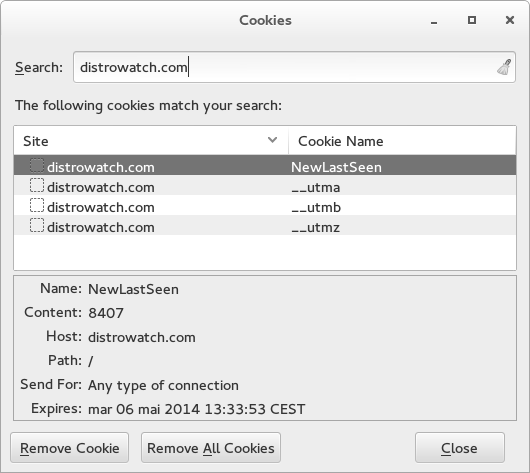
\includegraphics[scale=0.7]{figures/cookies_distrowatch_NB.png}
	\caption{\label{cookies_distrowatch}Les cookies enregistrés pour l'hôte \textit{distrowatch.com} dans Firefox.}
\end{figure}


%%%%%%%%%%%%%%%%%%%%%%%%%%%%%%
\section{Comment le Web est-il censé fonctionner ?}
Lors du chargement d'une page web, le navigateur effectue de multiples connexions afin de récupérer l'ensemble des ressources de la page. Aux débuts du World Wide Web, toutes les ressources d'une page appartenaient généralement à une même personne/groupe. A l'heure actuelle, la situation a fortement changé : il est fréquent de voir des ressources chargées depuis des domaines tiers (régies publicitaires, CDN,...). Le navigateur effectue donc des connexions vers des serveurs différents (cela permet notamment de passer outre la limitation du nombre de connexions HTTP vers un même domaine \cite{IETF_RFC2616}). En contrepartie, cela permet aux serveurs en question d'enregistrer des données sur le client suite aux requêtes qu'il effectue.


%%%%%%%%%%%%%%%%%%%%%%%%%%%%%%
\section{Principe de même origine}
\label{sop}
Le principe de même origine (\textit{same-origin principle}) peut être déclaré comme suit : "\textit{seul le site qui enregistre des données dans le navigateur peut lire ou modifier ces données plus tard}" \cite{Jackson:2006:PBS:1135777.1135884}. Son but est d'isoler des sites en respectant leur capacité à lire ou modifier l'état du navigateur. Cela permet à un utilisateur de naviguer comme si chaque site et chaque session étaient complètement indépendants.
\newline

Lors du développement de Netscape Navigator 2, une décision importante a été prise concernant le principe de même origine. Celui-ci interdit des sites web de domaines différents d'interagir entre eux au niveau du cache du navigateur, sauf dans des cas précis. Plus concrètement, son but est de permettre aux cookies et au JavaScript de sites web de confiance variable de coexister silencieusement dans le navigateur de l'utilisateur, sans interférer mutuellement. Ce principe est désormais implémenté dans les différents navigateurs mais il n'est pas appliqué de la même manière. En effet, le principe n'a ni été déclaré de manière générale ni appliqué de manière uniforme aux multiples façons dont un site web peut sauvegarder ou récupérer des données sur la machine d'un utilisateur.
\newline

Il n'est pas facile de déterminer quelles actions devraient être sujettes à un contrôle de sécurité \cite{zalewski2012tangled}. Il semble clair que certaines interactions, comme suivre un lien, devraient être permises sans restrictions spéciales étant donné qu'elles sont essentielles à la santé de l'environnement Web. En effet, c'est le principe même sur lequel repose le Web avec les liens hypertextes. A l'opposé, d'autres interactions, comme modifier le contenu d'une page chargé dans une autre fenêtre, devraient subir un contrôle de sécurité.

L'origine telle que définie selon le principe de même origine est le triplet protocole-hôte-port. Différents exemples issus du site de Mozilla \footnote{Mozilla est le développeur du navigateur Firefox.} sont disponibles dans la \autoref{origin_sop}.

\begin{figure}[h]
	\centering
		\begin{tabular}{|l|c|c|}
			\hline
			URL & Résultat & Raison \\
			\hline
			http://store.company.com/dir2/other.html		& Succès	& /						\\
			http://store.company.com/dir/inner/another.html	& Succès	& /						\\
			https://store.company.com/secure.html			& Echec		& Protocole différent	\\
			http://store.company.com:81/dir/etc.html		& Echec		& Port différent		\\
			http://news.company.com/dir/other.html			& Echec		& Hôte différent		\\
			\hline
		\end{tabular}
	\caption{\label{origin_sop}Différents exemples d'URL et leur comparaison par rapport à \mbox{\textit{http://store.company.com/dir/page.html}} selon le principe de même origine \cite{same_origin_policy_mozilla}.}
\end{figure}

La simplicité du principe de même origine est à la fois une aubaine et une malédiction \cite{zalewski2012tangled}. Son mécanisme est facile à comprendre et pas trop compliqué à implémenter mais son inflexibilité peut être une limite pour les développeurs. Il est parfois trop vaste, rendant impossible l'isolation de pages à des utilisateurs différents (à moins de faire un sous-domaine pour chaque utilisateur) et il peut rendre le partage d'informations difficile pour des sites coopérant de façon légitime (entre \textit{login.exemple.com} et \textit{paiements.exemple.com} par exemple).

\section{Conclusion}
Comme nous avons pu le voir dans ce chapitre, le protocole HTTP a été amélioré au fil du temps grâce à de nouvelles fonctionnalités. La plus importante d'entre elles est la possiblité pour le serveur de garder de l'information entre des requêtes HTTP successives issues d'un client. Sans cette fonctionnalité, le Web tel qu'on le connaît aujourd'hui n'existerait pas. Cependant, lorsque ces mécanismes ont été mis en place, la situation était différente et les aspects liés à la vie privée n'étaient pas encore d'actualité. Il en résulte que ces mécanismes ne proposent pas de solution adéquate afin d'éviter certaines attaques et c'est la raison pour laquelle le respect de la vie privée est un thème qui a attiré davantage l'attention au fil du temps.


\chapter{Moyens d'identification}
Dans ce chapitre, nous allons nous intéresser aux techniques qui permettent de tracer les utilisateurs. Plus précisément, nous allons voir comment ces techniques utilisent ou détournent les mécanismes assurant le fonctionnement du Web.

\section{Imperfections du principe de même origine}
\label{imperfections_sop}
L'échec de la bonne adaptation de ce principe est une source importante de fuites de données et d'attaques. Les violations du principe de même origine peuvent être dues à un filtrage de script insuffisant du côté des applications Web du serveur ou à des défauts dans les mécanismes d'isolation des domaines au sein du navigateur \cite{Chen:2007:ABD:1315245.1315248}.

Les défauts de filtrage des scripts au niveau des serveurs sont communément appelés failles XSS (\textit{cross-site scripting}). En exploitant ces failles, des scripts malveillants peuvent passer à travers le filtrage et être exécutés dans le même contexte de sécurité que les applications Web authentiques.

Au niveau des navigateurs Web, les violations du principe de même origine sont dues à une mauvaise isolation des contenus des différents domaines. Certains domaines peuvent alors accéder aux informations appartenant à d'autres domaines alors qu'ils ne devraient pas y avoir accès.
\newline

Lorsqu'un attaquant désire compromettre une application, il est parfois plus facile d'attaquer les utilisateurs à travers leur navigateur Web que le serveur lui-même \cite{sullivan2011web}. Les navigateurs sont défendus par le principe de même origine mais la présence de failles dans le site Web ou dans le serveur peuvent permettre à l'attaquant de passer outre ce principe. La principale vulnérabilité des sites sont les attaques XSS. Celles-ci permettent à un attaquant de placer son code au sein des pages d'une application Web vulnérable. Lorsqu'un visiteur se rend sur l'une de ces pages, le code de l'attaquant est chargé avec les autres éléments de la page. Ce script malicieux peut alors être en mesure de lire le cookie de l'utilisateur ou récupérer des valeurs affichées uniquement à l'utilisateur en utilisant du JavaScript. Ensuite, une requête HTTP contenant les données volées serait utilisée afin de les envoyer au serveur de l'attaquant. Celui-ci serait ensuite capable de se faire passer pour l'utilisateur légitime sur le site ou d'utiliser les informations reçues à mauvais escient (il pourrait par exemple s'agir de données bancaires), voir \autoref{exemple_XSS}.
\newline

\begin{figure}[h]
	\centering
	\begin{lstlisting}
<script>
  // Vol du numero de client
  var numeroDuClient = document.getElementById('numClient').innerHTML;
  // Vol du cookie
  var cookieDuClient = document.cookie;
  // Requete contenant les informations volees :
  var requete = 'http://serveur-du-voleur.be/vol?client=' + numeroDuClient + '&cookie=' + cookieDuClient;
  // Envoi de la requete avec une image
  document.write("<img src='" + requete + "'/>");
</script>
	\end{lstlisting}
	\caption{\label{exemple_XSS}Un exemple d'attaque XSS pour voler des informations.}
\end{figure}
Quand le client va se rendre sur la page, son navigateur va automatiquement faire une requête vers le serveur du voleur. Son navigateur l'avertira seulement que l'image n'a pas été trouvée mais les informations auront été néanmoins transmises au voleur. Cette attaque nécessite un minimum de préparation car le voleur doit savoir quel est le nom ou l'ID de l'élément HTML qui affiche le numéro de client (dans l'exemple, "numClient").
Ceci est un premier exemple de violation du principe de même origine réalisé avec l'aide d'une faille XSS.
\newline

Il existe plusieurs moyens de contourner le principe de même origine. Le but de ce chapitre n'étant pas d'en faire une liste exhaustive, seuls quelques moyens seront expliqués.
Il faut également préciser que même si le principe était correctement implémenté au sein d'un navigateur, il n'empêcherait pas les violations de vie privée face à des sites coopérants. Ceci s'explique par le fait qu'il existe une multitude de techniques simples allant des redirections jusqu'aux liens inter-sites pouvant être utilisées dans le but de transmettre des données entre des sites. Avec de tels échanges, les sites coopérants sont dans la capacité de constituer un profil inter-domaine des activités de leurs visiteurs.
%\newline

%La possibilité de violer le principe de même origine est la source de nombreuses méthodes qui permettent de tracer les utilisateurs. En effet, elle permet à un site A de créer et récupérer un cookie sur l'ordinateur de l'utilisateur s'il visite un autre site B qui inclut du contenu du site A (\autoref{cookies}). Cela autorise également des sites à accéder à des éléments d'un autre site enregistrés en cache (\autoref{cache}).

%L'absence d'implémentation du principe de même origine dans l'historique de l'utilisateur permet de déterminer si le navigateur a été utilisé pour visiter un site en regardant la couleur des liens hypertextes pointant vers ce site. Dans ce cas, l'utilisation de cookies n'est même plus nécessaire.
%\newline

%Le traçage des utilisateurs peut être classé en plusieurs catégories \cite{Jackson:2006:PBS:1135777.1135884} :
%\begin{itemize}
%  \item tracking sur une seule session : inévitable vu comment le Web fonctionne
%  \item tracking sur de multiples sessions : permet à un site d'identifier un visiteur s'il revient plus tard sur le site
%  \item tracking coopératif : permet à des sites coopérants de créer un historique des visites d'un utilisateur sur tous les sites de la coopération
%  \item tracking semi-coopératif sur un seul site : permet à un site de déterminer des informations sur les activités d'un visiteur sur un autre site en y plaçant du contenu (par exemple, en plaçant une image sur un forum)
%  \item tracking semi-coopératif sur de multiples sites : identique au tracking semi-coopératif sur un seul site à l'exception qu'il peut y avoir plusieurs sites ciblés
%  \item tracking non coopératif : permet à un site de déterminer des informations sur les activités d'un visiteur sur un autre site sans participation du site ciblé
%  \newline
%\end{itemize}
%
%Certains types de tracking peuvent être évités en améliorant le principe de même origine mais il est malheureusement difficile de contrer les types de tracking dits coopératifs.

%%%%%%%%%%%%%%%%%%%%%%%%%%%%%%
\section{Cookies}
\label{cookies}
En général, on utilise deux types de classification pour les cookies \cite{Yue:2007:ACU:1251984.1253093}.

Le premier se base sur l'origine et la destination : les cookies sont classifiés en tant que cookies "first-party" ou "third-party". Les cookies "first-party" sont issus du domaine que l'utilisateur est en train de visiter, on les appelle cookies d'origine ou cookies de domaine. Les cookies "third-party" sont créés par un site autre que celui qui est visité par l'utilisateur, on les appelle cookies tiers.\\
Les cookies tiers sont placés suite à des réponses HTTP venant de sites tiers. Un site \textit{alpha.com} ne peut pas créer de cookie au nom du site \textit{beta.com} (voir RFC 6265 \cite{IETF_RFC6265}, section 4.1.2.3), cela provoquerait des problèmes de sécurité évidents. Pour les mêmes raisons, les cookies ayant un suffixe public \footnote{Un suffixe public est un domaine qui est contrôlé par un registre public comme "com", "co.uk" ou "pvt.k12.wy.us" \cite{IETF_RFC6265}. Une liste est maintenue par le projet Mozilla : \url{http://publicsuffix.org/}.} dans l'attribut \textit{Domain} sont rejetés.

La seconde méthode de classification se base sur la durée de vie du cookie : les cookies sont alors classifiés en cookies de session ou cookies persistants. Les cookies de session sont stockés dans la mémoire vive de l'ordinateur et supprimés à la fermeture du navigateur. A l'opposé, les cookies persistants sont stockés sur le disque dur de l'ordinateur et supprimés soit lors de leur expiration, soit manuellement par l'utilisateur.
\newline

Les cookies tiers, qu'ils soient de session ou persistants, n'apportent quasiment aucun bénéfice à l'utilisateur. Ils sont d'ailleurs reconnus comme une menace pour la vie privée et les navigateurs proposent généralement une option pour les désactiver.

Les cookies d'origine de type session ne posent généralement pas vraiment de problèmes relatifs à la vie privée étant donné leur faible durée de vie. En théorie, ceci est valable car l'utilisateur ferme les fenêtres de son navigateur régulièrement. Par contre, un utilisateur qui laisse constamment l'onglet d'un site ouvert pourrait se faire tracer par le site en question.

A l'opposé, les cookies d'origine persistants peuvent poser des problèmes divers. En effet, les cookies persistants sont une arme à double tranchant : ils peuvent jouer un rôle utile en permettant la personnalisation et l'authentification sur les sites mais ils peuvent également jouer un rôle plus dangereux qui amène des risques au niveau de la vie privée et de la sécurité. Ces risques reposent sur deux aspects : le premier, et celui qui nous intéresse principalement ici, est que les cookies persistants permettent de tracer l'activité de l'utilisateur dans le temps. En effet, pour chaque page visitée, le client envoie une requête au serveur, celui-ci est donc capable de suivre l'utilisateur lors de la visite du site. Le deuxième risque est que les cookies persistants peuvent être volés ou manipulés par des attaques de deux types : les attaques XSS (elles exploitent les vulnérabilités des applications Web, voir la \autoref{exemple_XSS} de la \autoref{imperfections_sop}) et les attaques qui exploitent les vulnérabilités des navigateurs Web (via notamment le contournement du principe de même origine).
\newline

Une étude menée sur plus de 5000 sites à propos de l'utilisation des cookies \cite{Yue:2007:ACU:1251984.1253093} a montré que les cookies d'origine persistants sont largement utilisés et que plus de 60\% sont réglés pour expirer plus d'un an après leur création.
\newline

Désactiver tous les cookies tiers et garder les cookies d'origine de type session est supporté par la majorité des navigateurs actuels. Le problème se situe au niveau des cookies d'origine persistants car on ne sait pas comment les gérer et déterminer s'ils sont utiles ou néfastes pour l'utilisateur.

%- parler des cookies de cache dans la section cookies ou dans la section cache ?

%%%%%%%%%%%%%%%%%%%%%%%%%%%%%%
\section{Cache}
\label{cache}
Le cache du navigateur permet d'enregistrer localement une copie des fichiers afin de ne pas devoir les recharger lors d'une visite ultérieure. Ce mécanisme est très utile car il permet d'économiser de la bande passante et du temps. Cependant, il donne la possibilité à des sites web de déterminer si leurs visiteurs ont visité un autre site auparavant.

\subsection{Tracking par mesure du temps}
Une méthode d'exploitation du cache à des fins de surveillance est détaillé par Felten et Schneider \cite{Felten:2000:TAW:352600.352606}.
Le principe est assez simple : il exploite le fait qu'un fichier présent en cache sera chargé beaucoup plus rapidement qu'un fichier qui ne l'est pas. Donc en mesurant le temps d'accès au fichier, il est possible de déterminer si une personne a déjà visité le site web (ou plus précisément, la page) qui utilise ce fichier. En effet, rien n'empêche un site web de charger un fichier hébergé par un autre site.
\newline

Imaginons que l'administrateur d'un site \emph{(alpha.com)} veuille savoir si ses visiteurs se sont également rendus sur un autre site \emph{(beta.com)}. La première chose qu'il doit faire est de se rendre sur le site qu'il veut cibler et choisir un fichier statique pouvant être mis en cache et qui est chargé par tout visiteur (un logo par exemple). Ensuite, le but est de mesurer le temps d'accès du fichier cible.

Le plus fiable et facile est d'utiliser un applet Java ou un code JavaScript qui va mesurer le temps de chargement du fichier à partir de son URL. Même si l'utilisateur a désactivé l'exécution de Java et de JavaScript, il est possible d'obtenir une mesure suffisamment précise en chargeant les fichiers suivants dans l'ordre :

\begin{enumerate}
  \item un fichier du site \emph{alpha.com}
  \item le fichier cible du site \emph{beta.com}
  \item un autre fichier du site \emph{alpha.com}
\end{enumerate}

En soustrayant les moments auxquels le serveur reçoit les requêtes des fichiers 1 et 3, l'administrateur du site \emph{alpha.com} est en mesure d'avoir une approximation du temps qu'il a fallu pour charger le fichier 2 (celui de \emph{beta.com}).

Il faut néanmoins respecter certains critères pour que cela fonctionne : forcer le chargement des fichiers de manière séquentielle et de manière invisible en n'altérant pas l'apparence de la page afin que le client ne remarque rien.
\newline

Il est possible d'améliorer la probabilité de distinguer correctement les succès des défauts de cache en effectuant différentes mesures, ce qui permet alors de raffiner les seuils de discrimination : refaire plusieurs fois la mesure d'un même fichier (à partir de la seconde tentative, le fichier sera présent dans le cache) pour les succès de cache et utiliser l'URL de fichiers n'existant pas pour les défauts de cache.

Afin d'améliorer la précision, il est également intéressant de combiner les résultats de plusieurs fichiers mesurés individuellement.
\newline

D'une manière semblable, ce type d'attaque peut également être réalisé sur le cache du DNS. Felten et Schneider ont vérifié la précision des tests avec l'aide de 3 serveurs distincts situés à des distances différentes.

Plus le serveur est situé à une grande distance, plus la requête DNS prend de temps. Les tests ont montré que la précision des résultats pouvait être inférieure car la pénalité suite à des défauts de cache était très petite. Il n'était donc pas possible de discriminer les échecs des succès de cache. Cependant, sur Internet, la pénalité en cas de défaut est suffisamment grande pour assurer une bonne distinction. Dans ce cas-là, les tests montrent une très bonne précision.
\newline

% Attache de cookies de cache

Cette attaque peut être menée dans différentes situations :
\begin{itemize}
  \item Un site web qui veut en savoir davantage sur ses visiteurs.
  \item Une régie publicitaire pourrait inclure le code de mesure dans les bannières qu'elle distribue afin de faire des statistiques sur les sites web consultés par les visiteurs.\\Il est même possible de distribuer un code différent pour les catégoriser.\\Bien entendu, cette attaque résulte d'une collaboration entre le site et la régie publicitaire.
  \item L'attaquant pourrait créer un site web de telle façon à ce qu'il apparaisse en tête des moteurs de recherche dans le but de faire des statistiques sur les personnes intéressées par un sujet particulier. Il faut noter que cette situation reste théorique et a peu de chances de fonctionner.
  \item L'attaquant pourrait envoyer un mail contenant le code HTML à sa victime.\\En le faisant ressembler à du spam, la victime ne remarquerait rien d'anormal et la mesure serait effectuée.
\end{itemize}

% Timing Attacks on Web Privacy (section 1) : raisons de s'inquiéter
% Timing Attacks on Web Privacy (section 7) : contre-mesures actuelles sont inefficaces
% Timing Attacks on Web Privacy (section 8) : solution possible

\subsection{Stockage local HTML5}
\label{cache_html5}
Une nouveauté d'HTML5 est la possibilité de stocker localement des données pour un usage hors-ligne \cite{West:2012:APS:2038772.2038791}.
Le stockage local pourrait servir de "super-cookie" car il permet de stocker jusqu'à 5MB de données. De plus, ces données sont dites persistantes car elles doivent être supprimées par l'utilisateur ou le site Web.
\newline

Dans une expérience portant à l'origine sur le traçage via les cookies Flash \cite{flash_cookies_privacy_2} (voir \autoref{flash}), les chercheurs ont ajouté cette nouvelle dimension apportée par l'HTML5.
L'expérience réalisée une première fois en 2009 portait sur les cookies Flash et les cookies HTTP. Une expérience similaire a été réalisée à nouveau en 2011 en apportant également des informations relatives au stockage permis par l'HTML5.
\newline

Les analyses ont été réalisées sur le TOP 100 donné par Quantcast \footnote{Quantcast est une entreprise spécialisée dans la mesure d'audience et la publicité.} en juillet 2011.
Il en ressort que 17 sites sur les 100 ont utilisé le stockage local HTML5 pour un total de 60 paires clé-valeur. Les chercheurs ont trouvé des correspondances entre le stockage local HTML5 et les cookies HTTP dans différents cas (\textit{twitter.com}, \textit{tmz.com}, \textit{squidoo.com}, \textit{nytimes.com}, \textit{hulu.com}, \textit{foxnews.com} et \textit{cnn.com}). Dans la plupart de ces cas, la valeur commune aux deux éléments était issue d'un service tiers (comme \textit{meebo.com}, \textit{kissanalytics.com} et \textit{polldaddy.com}).

\subsection{ETags}
\label{cache_etags}
Le champ d'entête \textit{ETag} est défini dans la RFC 2616 \cite{IETF_RFC2616}. Il permet de déterminer si l'élément présent en cache dans le navigateur correspond à celui présent sur le serveur. Il est choisi arbitrairement par le serveur et est placé dans les réponses HTTP. Lorsqu'un client fait une requête vers un serveur et qu'il possède une copie du fichier en cache avec son \textit{ETag}, le serveur va comparer les deux \textit{ETags}. Cela permet d'économiser de la bande passante car le serveur n'envoie pas l'élément si les deux \textit{ETags} correspondent. Un exemple est disponible à la \autoref{etag} \footnote{Exemple basé sur \url{http://www.w3.org/2005/MWI/BPWG/techs/CachingWithETag.html}}.
\begin{figure}[h]
	\centering
	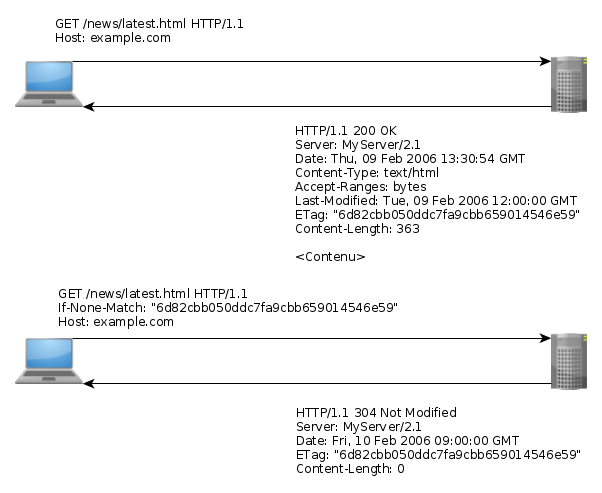
\includegraphics[scale=0.6]{figures/ETag.png}
	\caption{\label{etag}Un exemple de requêtes et réponses HTTP utilisant l'\textit{ETag}.}
\end{figure}
\newline

Dans l'expérience mentionnée dans la \autoref{cache_html5} et expliquée dans la \autoref{flash}, les chercheurs ont trouvé un cas de réapparition de cookie HTTP (un cookie HTTP a été supprimé par l'utilisateur puis un cookie identique a été recréé grâce au stockage local HTML5) sur \textit{hulu.com} à travers un service hébergé sur \textit{kissmetrics.com}. La technique a utilisé les ETags afin de sauvegarder les valeurs.
\newline

D'après les chercheurs, le tracking via l'entête ETag et le fait de pouvoir recréer des cookies à l'identique est particulièrement problématique car cette technique génère des valeurs de tracking uniques même si l'utilisateur bloque les cookies HTTP et Flash. En effet, afin d'empêcher ce traçage, l'utilisateur devrait vider son cache entre chaque site visité. De plus, en mode de navigation privée, l'utilisateur peut quand même être suivi durant une même session \cite{flash_cookies_privacy_2}.

%%%%%%%%%%%%%%%%%%%%%%%%%%%%%%
\section{Pixels espions}
\label{pixels_espions}
Les pixels espions sont des images de taille minime (généralement, de 1 pixel de haut sur 1 pixel de large) et sont destinés à effectuer une requête HTTP vers un serveur sans que le visiteur de la page ne s'en aperçoive. L'administrateur du site hébergeant ce pixel espion peut dès lors analyser les logs de son serveur Web afin d'obtenir des informations sur l'utilisateur. En plaçant un pixel espion spécifique sur chaque site, il est possible de distinguer sans problème les requêtes provenant des différents sites et ainsi déterminer quel site a été visité par chaque utilisateur.
En analysant la requête envoyée par le client, le serveur peut connaître plusieurs informations : la date et l'heure à laquelle le visiteur s'est rendu sur la page, son "User-Agent" (le navigateur utilisé, sa version, le système d'exploitation,...), la langue, les cookies et toutes les informations disponibles par défaut dans une requête HTTP.\\
De plus, l'URI présente dans celle-ci peut contenir des informations additionnelles placées dans la chaîne de requête de l'URI (après le point d'interrogation), comme cela est illustré dans la \autoref{exemple_XSS}.
\newline

Les pixels espions sont généralement utilisés pour tracker les visites. Par exemple, un site commercial pourrait placer un pixel de tracking sur sa page de confirmation d'achat. Cela enverrait alors une requête vers un serveur qui analyse les requêtes reçues et le parcours de l'acheteur pourrait être retracé avec l'information contenue dans le cookie. Par exemple, un cookie pourrait contenir le nom de la campagne de publicité qui a amené le visiteur sur le site. Les statistiques reçues permettraient alors au site de déterminer quelle campagne marketing a le mieux fonctionné.

%%%%%%%%%%%%%%%%%%%%%%%%%%%%%%
\section{JavaScript}
\label{JavaScript}
JavaScript permet d'exécuter des scripts du côté client. Il a entraîné le déploiement d'applications riches et accessibles simplement via un navigateur Web. Les possibilités sont multiples : il est ainsi facile de se divertir grâce à un jeu écrit en JavaScript mais il est également aisé d'en savoir plus sur l'utilisateur via le navigateur qui exécute le script. Ceci est possible grâce à l'accès dont dispose JavaScript sur l'ordinateur du client. En effet, différentes attaques peuvent être perpétrées avec JavaScript afin d'identifier les utilisateurs \cite{Jang:2010:ESP:1866307.1866339} :

\begin{itemize}
	\item Le vol de cookies : le script inclus depuis un site tiers peut accéder à toutes les informations présentes sur la page. Lorsque celle-ci fait appel à un script, elle lui donne accès aux cookies, à la barre d'adresses et à l'ensemble des éléments disponibles sur la page. Le script a donc la capacité de lire le contenu des cookies associés au site et de l'envoyer à un site tiers.% (une régie publicitaire par exemple).
	\item Le détournement d'adresse : le script, ayant l'accès complet au contenu de la page, peut influencer les valeurs des URL. Le script peut également rediriger le navigateur vers un autre site et le ramener ensuite vers le site d'origine sans que l'utilisateur ne s'en aperçoive (au chargement de la page par exemple).
	\item L'analyse de l'historique : l'attaque consiste à regarder comment les liens sont affichés par le navigateur. En effet, s'ils ont été visités, les liens s'affichent d'une autre couleur. Avec JavaScript, il suffit alors de créer un lien vers le site que l'on désire cibler dans une partie invisible de la page et utiliser l'interface DOM du navigateur pour regarder comment celui-ci affiche le lien. Cette attaque est possible car dans la plupart des navigateurs, l'accès à un historique de pages visitées, de fichiers cachés et de cache DNS est partagé entre les domaines. Cependant, ces éléments ne sont pas accessibles simplement. Par exemple, il est nécessaire de placer un lien vers un site pour accéder à l'information concernant ce site et pouvoir déterminer s'il a été visité grâce à la couleur du lien affiché.
	\item Le traçage de comportement : il est possible de déterminer avec précision le comportement de l'utilisateur sur la page qu'il visite. L'élaboration d'une ligne du temps avec les interactions de l'utilisateur (clics, mouvements, défilements, parties de texte surlignées,...) est réalisable avec l'aide de gestionnaires d'événements. Cet ensemble d'interactions peut alors être envoyé à un site tiers afin de calculer des statistiques sur la navigation de l'utilisateur.
	\newline
\end{itemize}

Lorsque du code JavaScript est inclus dans une page, il n'est pas soumis au principe de même origine (\autoref{sop}). Ce script a donc accès à l'ensemble des éléments de la page et pourrait potentiellement récupérer des données, voir \autoref{inclusion_js}. \cite{sullivan2011web}.
\begin{figure}[h]
	\centering
	\begin{lstlisting}
<script src="http://exemple.com/script.js />
	\end{lstlisting}
	\caption{\label{inclusion_js}Inclusion d'un code JavaScript dans une page.}
\end{figure}

Une propriété de JavaScript mérite aussi notre attention, il s'agit de \textit{document.domain}. Cette propriété permet à deux sites ayant le même domaine de plus haut niveau de s'accorder sur le fait qu'ils veulent être considérés équivalents. Par exemple, afin de pouvoir s'échanger des données, deux sites \textit{login.exemple.com} et \textit{paiements.exemple.com} pourraient passer outre la vérification habituelle du domaine (les protocoles et les ports doivent correspondre), voir \autoref{js_document_domain}.
\begin{figure}[h]
	\centering
	\begin{lstlisting}
document.domain = "exemple.com"
	\end{lstlisting}
	\caption{\label{js_document_domain}Modification du domaine de la page avec JavaScript.}
\end{figure}

\subsection{Régies publicitaires sur Internet}
Il semble logique que les régies publicitaires se soient intéressées au tracking des utilisateurs. Grâce à lui, elles sont en mesure de calculer des statistiques diverses sur les intérêts des utilisateurs, ceci ayant pour but de les inciter à consommer davantage en leur proposant par exemple des produits qui ont plus de chances de les intéresser. Le tracking leur permet également de calculer les montants que leurs clients vont payer (pour ceux qui affichent les publicités de leurs produits) ou recevoir (pour ceux qui affichent de la publicité sur leur site). Ainsi, Google possède 2 services : \textit{Google Adsense} qui utilise les contenus des utilisateurs (sites Web, vidéos YouTube,...) comme support d'affichage pour les publicités et \textit{Google Adwords} qui propose à des annonceurs de diffuser leurs publicités.
\newline

Les techniques utilisées par les régies publicitaires sont globalement les mêmes que pour les autres entreprises : il faut inclure un code JavaScript qui va s'occuper de faire le tracking des utilisateurs et ce code contient généralement l'identifiant du client de la régie publicitaire. Il faut noter que les régies publicitaires sont parfois prêtes à aller loin pour s'assurer du suivi des utilisateurs. C'est pourquoi certaines n'hésitent pas à user de techniques malicieuses pour recréer des cookies HTTP effacés grâce à Flash ou au stockage local HTML5 (voir les sections correspondantes).
\newline

La publicité sur Internet constitue un important modèle économique qui supporte l'accès gratuit à une majorité de contenus. Afin de pouvoir gagner un profit, les éditeurs placent des publicités sur leur site et se font payer par des publicitaires ou réseaux publicitaires. Vu la popularité du Web aujourd'hui, ces derniers veulent que leurs techniques soient de plus en plus sophistiquées. Au lieu d'afficher la même publicité chez tous les utilisateurs, ils souhaitent que leurs publicités soient personnalisées. Afin de parvenir à faire de la publicité ciblée, ils doivent être en mesure de déterminer le profil de chacun et c'est pour cela que le traçage des utilisateurs semble s'intensifier avec le temps \cite{Tran:2012:TTF:2352593.2352627}.

\subsection{Modules des réseaux sociaux}
Les réseaux sociaux proposent généralement de placer un module social qui permet aux visiteurs d'un site d'interagir et de partager avec leurs amis. Bien sûr, l'intégration d'un tel script permet aux plateformes de réseaux sociaux de suivre la navigation des visiteurs d'un site. Si beaucoup de sites intègrent ces scripts, les réseaux sociaux sont alors en mesure d'obtenir une sorte de carte d'Internet avec les déplacements et actions de chaque utilisateur. En effet, à chaque page contenant un module social, une requête est effectuée vers le serveur du réseau social ; celui-ci peut donc le suivre. De plus, si le visiteur est connecté à son compte sur le réseau social en naviguant sur d'autres sites, la plateforme peut directement faire le lien entre son profil et les sites qu'il visite.
\newline

Les principaux réseaux sociaux proposent généralement les mêmes fonctionnalités. Celles-ci sont également disponibles sur différents systèmes d'exploitation tels qu'Android ou iOS.

\begin{figure}[h]
	\centering
	
\includegraphics[scale=0.6]{figures/modules_sociaux_lesoir.png}
	\caption{Partage via les modules des réseaux sociaux sur \textit{lesoir.be}.}
\end{figure}

\begin{figure}[h]
	\centering
	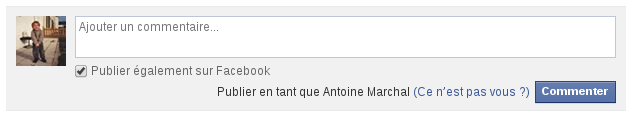
\includegraphics[scale=0.6]{figures/module_facebook_lalibre.png}
	\caption{Module de commentaires via Facebook sur \textit{lalibre.be}.}
\end{figure}

\begin{figure}[h]
	\centering
	
\includegraphics[scale=0.6]{figures/module_facebook_lesoir.png}
	\caption{Module incitant le visiteur à lier son compte Facebook au site \textit{lesoir.be}.}
\end{figure}

\subsubsection{Facebook}
Le code que les gestionnaires de sites Web doivent intégrer au sein de leur page afin d'accéder aux fonctionnalités offertes par Facebook \cite{javascript_facebook_sdk} est visible à la \autoref{js_facebook_sdk}. L'intégration de ce code permet aux sites Web d'utiliser entre autres les plugins suivants : le bouton "Like", le bouton de partage, le flux d'actualités d'une page Facebook et le module de commentaires.

Facebook propose également un SDK pour PHP et donne une liste de SDK, plugins et outils développés par d'autres. Les possibilités offertes par Facebook sont nombreuses, elles vont du module d'identification au module de paiement en passant par la publicité. Tout est bien détaillé sur un portail destiné aux développeurs \footnote{\url{https://developers.facebook.com/docs/}}.

\begin{figure}[h]
	\centering
	\lstinputlisting{examples/js_facebook_sdk}
	\caption{\label{js_facebook_sdk}Le SDK de \textit{Facebook} pour JavaScript.}
\end{figure}

\subsubsection{Google+}
De son côté, Google propose différents scripts à ajouter en fonction des fonctionnalités que le gestionnaire de site web veut intégrer au sein de sa page (voir \autoref{js_google_plus}). Google propose même de charger de façon asynchrone son script afin d'obtenir des performances optimales (voir \autoref{js_google_plus_async}) \cite{javascript_google_plus}. Google+ propose le même genre de plugins \footnote{\url{https://developers.google.com/+/}} que Facebook tels que l'installation d'un module d'identification par compte Google, des boutons de partage, de recommandations, de suivi et autres.

\begin{figure}[h]
	\centering
	\lstinputlisting{examples/js_google_plus}
	\caption{\label{js_google_plus}L'API JavaScript de \textit{Google+}.}
\end{figure}

\begin{figure}[h]
	\centering
	\lstinputlisting{examples/js_google_plus_async}
	\caption{\label{js_google_plus_async}L'API JavaScript de \textit{Google+} pour un chargement asynchrone.}
\end{figure}

\subsubsection{LinkedIn}
LinkedIn propose également une API pour connecter les sites avec sa plateforme \cite{javascript_linkedin}. Dans la \autoref{js_linkedin}, on peut même voir que le nom de l'utilisateur (s'il est connecté sur la plateforme) est affiché sur le site. Cet aspect semblera convivial à la majorité des utilisateurs mais cela permet surtout de mieux les suivre lors de leur navigation sur les sites intégrant ce module social. Cette fonctionnalité est d'ailleurs également proposée par les autres plateformes de réseaux sociaux.

\begin{figure}[!h]
	\centering
	\lstinputlisting{examples/js_linkedin}
	\caption{\label{js_linkedin}L'API JavaScript de \textit{LinkedIn}.}
\end{figure}

\subsection{Outils destinés aux webmasters}
Certaines plateformes proposent aux gestionnaires de sites Web de suivre la navigation des visiteurs sur leur site. Elles regardent d'où viennent les visites (moteur de recherche, accès direct, lien d'un autre site,...), leur navigateur (la version, les extensions installées, la langue,...), sur quelles pages les visiteurs se rendent, le temps passé sur chaque page, etc.

\subsubsection{Google Analytics (Universal Analytics)}
\label{google_analytics}
Une des principales plateformes de suivi des utilisateurs est Google Analytics. Cet outil est utilisé par de nombreux gestionnaires de sites afin de connaître les statistiques de fréquentation de leur site \cite{javascript_google_analytics}. Les webmasters doivent inclure le code JavaScript de la \autoref{js_google_analytics} afin de pouvoir utiliser cet outil.
\newline

\begin{figure}[!h]
	\centering
	\lstinputlisting{examples/js_google_analytics}
	\caption{\label{js_google_analytics}L'API JavaScript de \textit{Google Analytics}.}
\end{figure}

Comme on peut le voir sur la \autoref{Google_Analytics_1}, les statistiques sont très détaillées. Dans la \autoref{Google_Analytics_2}, la ville des visiteurs était affichée mais il est également possible de voir d'autres données telles que leur FAI ou leur système d'exploitation. Des données spécifiques aux clients mobiles sont également disponibles. Toutes les données sont affichées dans des graphiques clairs et dynamiques et il est même possible d'exporter l'ensemble de ces données dans différents formats (CSV, TSV, Excel, PDF,...) afin de les traiter de manière automatique.
%\newline

\begin{figure}[!h]
	\centering
	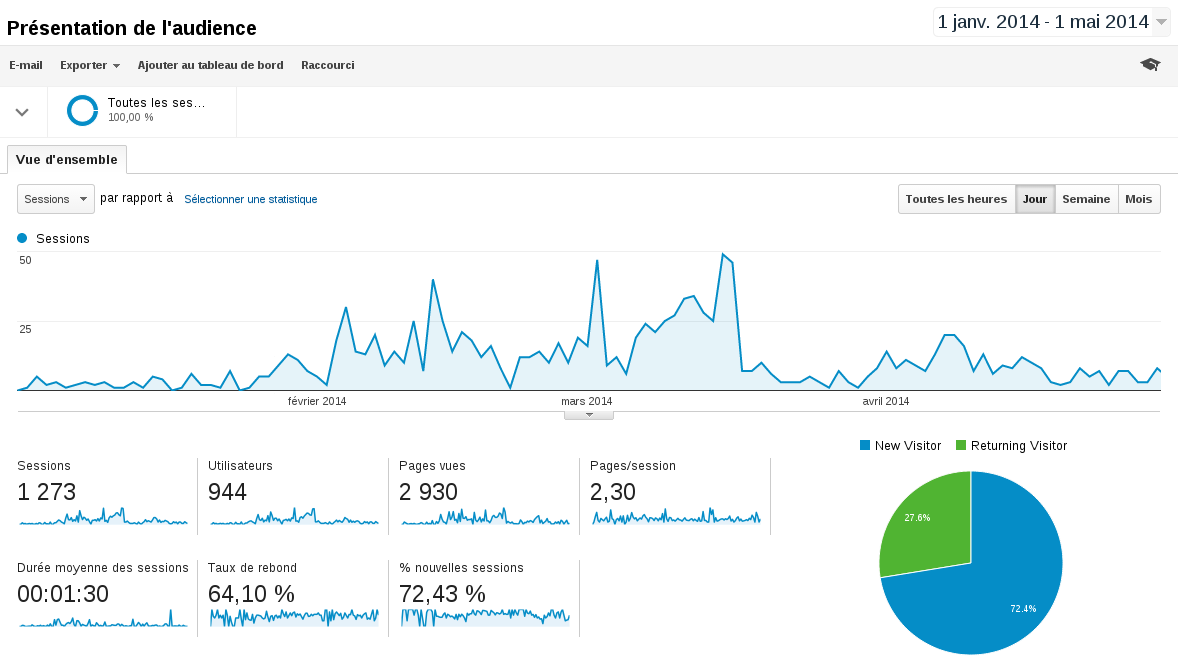
\includegraphics[scale=0.36]{figures/Google_Analytics_1.png}
	\caption{\label{Google_Analytics_1}Copie d'écran de \textit{Google Analytics} qui détaille les visites.}
\end{figure}

\begin{figure}[!h]
	\centering
	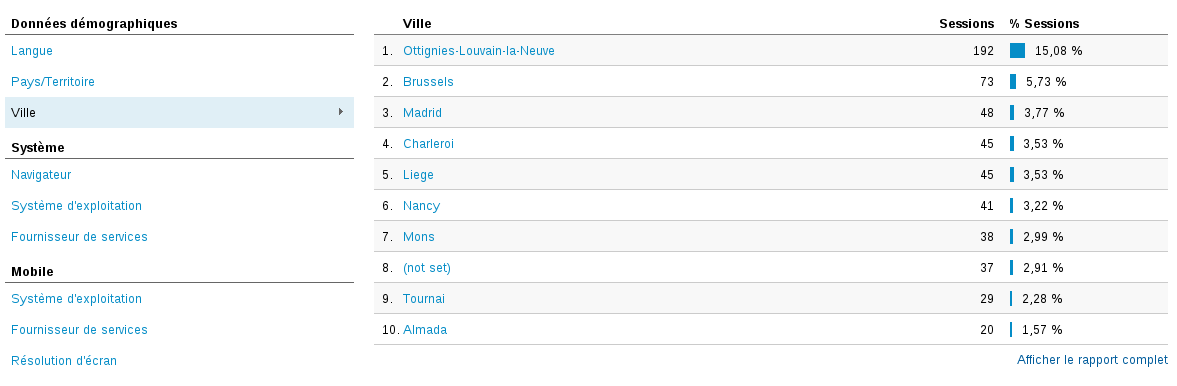
\includegraphics[scale=0.36]{figures/Google_Analytics_2.png}
	\caption{\label{Google_Analytics_2}Copie d'écran de \textit{Google Analytics} qui détaille l'origine des visiteurs.}
\end{figure}

Google a développé une nouvelle version de son outil d'analyse des visiteurs : Universal Analytics. Ce nouvel outil repose sur le même socle que Google Analytics mais il apporte de nouvelles fonctionnalités.
\newline
\newpage

Pour ce nouvel outil, Google propose 3 types de code de tracking en fonction des plateformes visées : la librairie JavaScript \textit{analytics.js} pour les sites Web, les SDK Google Analytics pour les applications mobiles et le \textit{protocole de mesure ("Measurement Protocol")} pour les autres appareils tels que consoles de jeux.% et les kiosques d'information.
\newline

Alors que Google Analytics identifiait un utilisateur différent en fonction de chaque appareil connecté, Universal Analytics reconnaît un même utilisateur qui utilise plusieurs moyens de se connecter à Internet. Afin d'y parvenir, Google utilise un identifiant d'utilisateur unique afin d'associer les données reçues d'appareils et de sessions différents.
\newline

Afin d'utiliser cette fonctionnalité, les gestionnaires de sites Web doivent être en mesure de générer un identifiant unique pour chaque utilisateur et l'associer aux données envoyées à Google. Généralement, cet identifiant unique est généré grâce à l'authentification des visiteurs sur un site. Ainsi, lorsqu'un utilisateur se sert de sa tablette et de son ordinateur pour se rendre sur un site et s'il s'y connecte, Google sera en mesure d'identifier ces visites comme provenant d'un seul et même utilisateur et non plus de deux utilisateurs différents.
\newline

En fonction de la version de Google Analytics utilisée, différents cookies sont créés et utilisés afin de suivre les visites des utilisateurs \cite{Google_Analytics_cookies}.
\newline

La nouvelle librairie JavaScript de Google, \textit{analytics.js} crée un cookie d'origine contenant un identifiant anonyme afin de distinguer les utilisateurs. Par défaut, la librairie crée un cookie sur le domaine de plus haut niveau et règle le chemin du cookie sur le niveau racine.
\newline

Le cookie créé est :
\begin{itemize}
  \item[$\bullet$] \textbf{\_ga} : cookie avec une date d'expiration de 2 ans destiné à distinguer les utilisateurs.
  \newline
\end{itemize}

L'ancienne libraire JavaScript de Google, \textit{ga.js}, crée 5 cookies d'origine qui permettent de :
\begin{itemize}
  \item déterminer quel domaine est mesuré
  \item distinguer les utilisateurs uniques
  \item se souvenir du nombre et des heures des visites précédentes
  \item se souvenir de l'information sur la source de trafic
  \item déterminer le début et la fin de session
  \item se souvenir des valeurs des variables personnalisées au niveau de l'utilisateur
  \newline
\end{itemize}

Par défaut, la librairie crée un cookie sur le domaine spécifié dans la propriété du navigateur \textit{document.host} et règle le chemin du cookie sur le niveau racine.
\newline

Les cookies créés sont:
\begin{itemize}
  \item[$\bullet$] \textbf{\_\_utma} : cookie avec une date d'expiration de 2 ans destiné à distinguer les utilisateurs et les sessions.
  \item[$\bullet$] \textbf{\_\_utmb} : cookie avec une date d'expiration de 30 minutes destiné à distinguer les nouvelles sessions et visites.
  \item[$\bullet$] \textbf{\_\_utmc} : cookie avec une date d'expiration de fin de session qui n'est plus utilisé dans \textit{ga.js} mais qui permet l'interopérabilité avec \textit{urchin.js} (une librairie encore plus ancienne de Google Analytics, antérieure à \textit{ga.js}).
  \item[$\bullet$] \textbf{\_\_utmz} : cookie avec une date d'expiration de 6 mois destiné à enregistrer les sources de trafic ou de campagne qui retrace comment un utilisateur atteint le site.
  \item[$\bullet$] \textbf{\_\_utmv} : cookie avec une date d'expiration de 2 ans utilisé pour sauvegarder les données des variables personnalisées au niveau de l'utilisateur.
  \newline
\end{itemize}

Avec le nombre élevé de sites utilisant les services de Google, ce dernier a les moyens de dresser une carte d'Internet. Il est même en mesure de connaître la plupart des sites visités par l'utilisateur (à la condition qu'ils intègrent un tracker de Google). Cela va sans dire que Google détient une très grande quantité d'informations sur les utilisateurs du Web actuel quand on y ajoute les messages privés (Gmail), la localisation (Android) et les nombreux autres services du groupe.

%%%%%%%%%%%%%%%%%%%%%%%%%%%%%%
\section{Flash}
\label{flash}
Adobe Flash Player \cite{flash_website} est un logiciel qui permet de lire du contenu multimédia. Il est notamment utilisé pour la conception de jeux sur Internet ou pour le streaming audio/vidéo (il était auparavant utilisé par YouTube qui a désormais décidé de se tourner vers la technologie HTML 5 \cite{youtube_html5}).
\newline

Flash peut être utilisé dans le tracking des utilisateurs car il utilise son propre système de cookies : les LSO (Local Shared Objects) \cite{conf/aaaiss/SoltaniCMTH10}. Ces derniers sont même considérés plus invasifs que les cookies HTTP car ils possèdent ces caractéristiques qui les rendent spéciaux \cite{flash_lso} :
\begin{itemize}
  \item ils permettent de stocker plus d'informations (100KB au lieu de 4KB pour les cookies HTTP)
  \item ils n'ont pas de date d'expiration par défaut
  \item ils sont stockés dans un emplacement différent, ce qui implique que la plupart des utilisateurs ne savent pas les effacer facilement et qu'ils sont accessibles via différents navigateurs
  \item ils ne sont pas contrôlés par le navigateur et celui-ci ne peut donc pas les effacer
  \item ils permettent de stocker des types de données simples (String, Array et Date)
  %\newline
\end{itemize}

Ces caractéristiques font que les cookies Flash (ce sont des fichiers avec l'extension \textit{.sol}) sont plus persistants et méconnus des utilisateurs. Pour supprimer les cookies Flash sans connaître leur emplacement, il faut se rendre sur une page dédiée \footnote{\url{http://www.macromedia.com/support/documentation/en/flashplayer/help/settings_manager07.html}} du site d'Adobe \footnote{Adobe est le développeur de Flash Player.}.
\newline

Le répertoire utilisé pour les stocker sur Linux est :\\
\mbox{\textit{/home/<user>/.macromedia/Flash\_Player}}. Celui-ci abrite deux répertoires :
\begin{enumerate}
  \item macromedia.com : il contient les paramètres de chaque site utilisant Flash.
  \item \#SharedObjects : il contient les LSO (les cookies Flash).
  %\newline
\end{enumerate}

Avec le contenu du répertoire \textit{macromedia.com}, on peut constater un autre risque de fuites concernant la vie privée : en analysant les traces laissées dans ce répertoire, il est possible de reconstituer une partie de l'historique de navigation de l'utilisateur. En effet, pour chaque domaine, un dossier est créé portant son nom et contenant un fichier de préférences \textit{settings.sol}. Simplement en regardant le nom des dossiers, il est possible de découvrir certains sites visités (voir \autoref{ls_macromedia.com}).

Notez que le navigateur Google Chrome n'utilise pas ce répertoire car Flash est intégré au navigateur \cite{flash_chrome}. Il est donc possible de supprimer les cookies Flash dans les paramètres du navigateur ou en se rendant sur la page dédiée du site Adobe.
\newline

\begin{figure}[h]
	\centering
	\lstinputlisting[style=dig]{examples/ls_macromedia.com}
	\caption{\label{ls_macromedia.com}Affichage des dossiers dans \textit{macromedia.com}.}
\end{figure}

Dans une expérience réalisée en 2009 \cite{conf/aaaiss/SoltaniCMTH10}, il a été montré que dans le TOP 100 des sites (classement Quantcast - juillet 2009), 54 sites ont utilisé des cookies Flash. Ces 54 sites ont généré 157 fichiers LSO pour arriver à un total de 281 cookies individuels. 98\% de ces sites ont également créé des cookies HTTP (seuls \textit{wikipedia.org} et \textit{wikimedia.org} ne l'ont pas fait) pour un total de 3602 cookies HTTP.
\newline

Ensuite, les chercheurs ont analysé les noms de variables les plus fréquemment utilisés dans ces cookies. Il en est ressorti que "volume" était en première position, ce qui fait penser à une préférence de volume pour le streaming (ce qui est logique car Flash reste avant tout un lecteur multimédia). Juste derrière et dans la majorité des cas, les noms de variables reflétaient l'idée d'identifiant (\textit{userid}, \textit{user}, \textit{id},...). Il est donc clair que les cookies Flash sont utilisés pour tracer les utilisateurs.
\newline

Le contenu des cookies Flash a été comparé avec le contenu des cookies HTTP. Sur les 100 sites, 31 montraient au moins un lien entre les cookies Flash et HTTP. Sur la totalité des 31 sites, 41 correspondances ont été trouvées.
\newline

Les chercheurs ont également montré que les cookies Flash étaient utilisés pour faire réapparaître les cookies HTTP lorsqu'ils étaient supprimés. Ainsi, certains sites recréaient les cookies HTTP grâce aux cookies Flash. Donc même si l'utilisateur effaçait les cookies HTTP via les préférences de son navigateur, les cookies de certains sites avec leur valeur étaient de nouveau envoyés lors des visites sur ces sites. Il faut également noter que certains cookies HTTP étaient recréés par des cookies Flash tiers.
\newline
\newpage

En 2011, l'expérience a été menée à nouveau \cite{flash_cookies_privacy_2}. Cette fois, les chercheurs se sont penchés également sur le stockage local HTML5 (voir la \autoref{cache_html5}). Les résultats sont les suivants : 5675 cookies HTTP ont été détectés (au lieu de 3602 en 2009). 20 sites ont placé 100 cookies ou plus et 7 sites en ont placé plus de 150. La plupart des noms de variables de ces cookies font penser à un identifiant unique de tracking. La plupart des cookies (4915) sont placés par un domaine tiers.

Concernant les cookies Flash, ils sont en baisse car 100 ont été détectés (au lieu de 281 en 2009) sur 37 sites (au lieu de 54 en 2009).
Deux sites (hulu.com et foxnews.com) utilisaient des valeurs communes dans leurs cookies Flash et HTTP, la valeur était également commune dans le stockage local HTML5.
\newline

Il faut noter qu'Adobe a condamné l'utilisation des LSO à des fins de tracking. L'entreprise incite les développeurs à utiliser la technologie Flash de manière responsable et de ne pas utiliser de technique qui permette d'utiliser le stockage local afin de recréer des cookies effacés par l'utilisateur sans son consentement \footnote{La déclaration complète d'Adobe est disponible à l'URL suivante : \url{http://www.ftc.gov/policy/public-comments/comment-544506-00085}}. Ils détaillent également quelques nouveautés qui ont été ajoutées aux versions ultérieures de Flash (notamment le support de la navigation privée).
\newline

Avant la version 10.1 de Flash Player \cite{flash_private}, celui-ci ne prenait pas en compte les effets des sessions de navigation privée des navigateurs. Cela signifie que lorsqu'un utilisateur activait une session de navigation privée avec son navigateur, les cookies, fichiers en cache et l'historique de sa session étaient supprimés par le navigateur mais ce n'était pas le cas pour les cookies Flash. Depuis la version 10.1 de Flash Player, celui-ci garde les fichiers LSO de la navigation privée en mémoire sans les enregistrer sur le disque et n'accède pas non plus aux LSO existants. A la fin de la session de navigation privée, Flash Player efface les données en conformité avec les préférences du navigateur.

%%%%%%%%%%%%%%%%%%%%%%%%%%%%%%
\section{Empreintes des navigateurs}
\label{fingerprinters}
Jusqu'à présent, nous avons vu des techniques de tracking dites avec état (stateful tracking). A l'opposé, il existe des techniques dites sans état (stateless tracking) utilisant des \textit{fingerprinters\footnote{En français, on pourrait traduire ce mot par "calculateur d'empreinte".}} \cite{Mayer:2012:TWT:2310656.2310703}. Ces derniers récupèrent une série d'informations qu'ils agrègent afin d'associer un identifiant (presqu') unique à l'utilisateur. Le principal avantage de cette méthode est que les informations dépendent peu de l'utilisateur.
En effet, avec des techniques utilisant des cookies, le tracking peut être rendu complexe par la suppression des cookies par l'utilisateur. A l'inverse, avec les fingerprinters, les informations récupérées sont relativement stables grâce à leur nature (numéro de version du navigateur, système d'exploitation, résolution d'écran, etc).
\newline

Le \textit{fingerprinter} regroupe les informations qui lui sont nécessaires via différentes sources \cite{Nikiforakis:2013:CME:2497621.2498133}. La première source est constituée des plugins populaires tels que Flash. Par exemple, lorsqu'on demande au navigateur la plateforme d'exécution sur une version 64 bits de Linux, il répond "Linux x86\_64" alors que si on demande la même information à Flash, il répond en indiquant la version complète du noyau Linux. Il est également possible de déterminer si l'utilisateur utilise un second écran. En effet, avec l'implémentation Linux du plugin Flash, lorsque la résolution est demandée, Flash renvoie comme résolution d'écran la somme des écrans individuels alors que le navigateur renvoie la résolution de l'écran sur lequel la fenêtre est affichée.

Les outils de fingerprinting s'adaptent également aux navigateurs des utilisateurs. Il a été montré qu'ils utilisent des propriétés spécifiques à certains navigateurs afin de récupérer certaines données. C'est notamment le cas avec Internet Explorer et les propriétés \textit{navigator.securityPolicy} et \textit{navigator.systemLanguage} \cite{Nikiforakis:2013:CME:2497621.2498133}.

Une autre source importante d'informations vient des polices de caractères utilisées. Cette information n'est pas directement disponible via les navigateurs et les \textit{fingerprinters} n'hésitent pas à utiliser des plugins comme Flash pour récupérer cette liste. De plus, certains \textit{fingerprinters} incluent un "plan B" lorsque Flash n'est pas disponible. Ils mesurent la taille d'un phrase prédéfinie avec la police utilisée par défaut si la police demandée n'est pas disponible. Ensuite, ils appliquent une police différente et mesurent la taille de la même phrase. Si la taille est identique, cela veut dire que la police n'est pas disponible chez l'utilisateur. Ils sont ainsi en mesure de déterminer une liste de polices installées chez l'utilisateur (avec l'inconvénient que les polices les plus rares ne sont pas détectées). Il faut noter que la présence de certaines polices rares permettent d'identifier un utilisateur avec une précision beaucoup plus importante \cite{Boda:2011:UTW:2341491.2341497}.

Flash est également utilisé pour détecter les proxys HTTP. C'est d'ailleurs la raison pour laquelle il est désactivé dans des applications sensibles à l'anonymat.

Une dernière source utilisée dans Internet Explorer provient des DLL chargées dans le navigateur. Certaines accèdent à des valeurs du registre Windows afin de transmettre des informations telles que les identifiants des disques durs, des paramètres TCP/IP, le nom de l'ordinateur, l'identifiant de produit d'Internet Explorer, la date d'installation de Windows, l'ID produit Windows Digital et les pilotes \cite{Nikiforakis:2013:CME:2497621.2498133}.
%\newline

Au sein du tracking sans état, on peut distinguer deux types d'utilisation du \textit{fingerprinting} : le \textit{fingerprinting actif} qui acquiert les informations de manière active grâce à l'utilisation de scripts ou de plugins et le \textit{fingerprinting passif} qui acquiert les informations de manière passive grâce au trafic réseau (les requêtes et réponses HTTP).
Le \textit{fingerprinting passif} est particulièrement problématique car il n'est pas détectable par le client. Un fingerprinter n'utilisant que du fingerprinting passif sera moins performant mais sera néanmoins en mesure de tracer certains types d'utilisateurs qui visitent le Web avec un navigateur qui est rarement modifié (pas d'installation d'extensions) et peu mis à jour.
\newline

Un aspect intéressant à analyser est la stabilité des empreintes des navigateurs. En effet, l'empreinte d'un navigateur peut être modifiée par différentes actions : mettre à jour le navigateur, mettre à jour un plugin, désactiver les cookies, installer une nouvelle police de caractères (ou une application qui contient des polices) ou connecter un second moniteur (ce qui change la résolution d'écran). Il semblerait que les empreintes calculées ne soient pas particulièrement stables mais le fait que le navigateur dévoile tant d'informations rend cette technique de tracking très intéressante. \cite{Eckersley:2010:UYW:1881151.1881152}

%%%%%%%%%%%%%%%%%%%%%%%%%%%%%%
\section{Conclusion}
Les moyens existants et mis en place dans le but de tracker les utilisateurs sont nombreux et divers. Certains restent relativement basiques alors que d'autres utilisent des techniques plus complexes. Certains sont conçus principalement dans le but d'effectuer un tracking sur un site particulier (les outils d'analyses de visites) alors que d'autres sont destinés à tracer les visiteurs sur de multiples sites (les régies publicitaires) afin de créer un profil des visiteurs.

Il semble que les possibilités et moyens de tracker les utilisateurs naviguant sur Internet évoluent rapidement. De nouvelles techniques apparaissent alors que d'autres sont peu à peu oubliées.


\chapter{Analyse des principaux sites web}
\section{Objectif de l'analyse}
Le but de l'analyse est de parcourir les sites les plus visités au monde d'après le classement Alexa \footnote{Alexa \cite{AlexaTop} est une entreprise qui appartient à Amazon et qui est principalement connue pour les statistiques qu'elle fournit sur le trafic Web dans le monde entier.}. Ensuite, déterminer s'ils contiennent des trackers et, le cas échéant, leur nature. Deux types d'expérience peuvent être menés :
\begin{enumerate}
	\item Le premier consiste en une analyse à long terme.
	\item Le second consiste en une analyse ponctuelle.
\end{enumerate}

Le premier type d'expérience a pour but de déterminer si les sites modifient leurs trackers au fil du temps.
Le second type permet d'avoir une image globale du niveau de traçage opéré par les principaux sites à un instant donné. Il donne également la possibilité de tester l'efficacité des extensions de navigateur qui affirment protéger la vie privée (voir \autoref{results_plugins}).

\section{Description de l'outil implémenté}
L'idée initiale était d'utiliser le framework \textit{fpdetective} \cite{Acar:2013:FDW:2508859.2516674}. C'est un framework conçu pour la détection et l'analyse d'outils (\textit{fingerprinters}, voir \autoref{fingerprinters}) qui créent des empreintes de navigateurs. Ce framework semblait prometteur mais son efficacité s'est révélée insuffisante et il ne fonctionnait pas correctement. En effet, aucun \textit{fingerprinter} n'était détecté alors que certains étaient manifestement présents sur plusieurs sites web visités.

Etant donné que \textit{fpdetective} ne pouvait fournir les résultats demandés, la création d'un outil dédié à cette tâche était nécessaire. De plus, cela permettait davantage de souplesse au niveau des décisions d'implémentation et du paramétrage de la recherche de trackers.
\newline

L'outil a été implémenté en Java. Il se compose de deux éléments : le \textit{crawler} qui visite les sites web et exporte leur contenu au format HTTP Archive (HAR) et le \textit{parser} qui traite les fichiers HAR en déterminant si les sites correspondants renferment des trackers.
L'outil a été développé sous Eclipse et est destiné à être utilisé sur Linux. Un exécutable JAR est également disponible.
La liste des options disponibles au lancement de l'outil est détaillé à l'\autoref{options_outil_implémenté}.
\newline

\subsection{Crawler}
\label{crawler}
\subsubsection{Choix d'implémentation}
Afin d'automatiser le navigateur et de parcourir les sites sans intervention humaine, \textit{Selenium} \footnote {\textit{Selenium} \cite{selenium_homepage} est une suite d'outils qui permet d'automatiser les navigateurs. On peut par exemple créer des scripts qui vont faire visiter un navigateur sur différents sites et effectuer plusieurs actions.} est utilisé dans le \textit{crawler}. Plus précisément, c'est le pilote \textit{FirefoxDriver} de \textit{Selenium} qui est utilisé. Il permet de lancer une instance de Firefox et d'interagir avec celle-ci.

La première implémentation traitait directement le code source de la page. Il était possible d'aller sur le moteur de recherche Google, de sélectionner le champ de recherche, de taper une requête et de récupérer le résultat. Cependant, le processus était assez lent et incomplet car on ne pouvait pas récupérer les requêtes et les réponses HTTP. On pouvait juste récupérer les éléments associés à des balises (par exemple, récupérer toutes les images via les balises de type \textit{<img>}, les scripts avec les balises \textit{<script>},...) mais tout n'était pas récupérable car certains éléments étaient chargés sans être identifiés.

Afin de pallier ce problème, la deuxième implémentation utilisait un proxy \footnote{Un proxy est un serveur qui sert d'intermédiaire afin d'accéder à un réseau et récupérer des ressources d'un autre serveur.} qui exportait le contenu du site au format HTTP Archive \footnote{HTTP Archive est un format ouvert qui permet d'exporter des échanges de données collectés par un outil de monitoring HTTP \cite{har_spec}.}. L'ensemble des requêtes et réponses HTTP était récupéré et enregistré dans un fichier. Le parcours du code source de la page (qui donnait des résultats finalement incomplets) a été supprimé afin de rendre le programme plus rapide. Cette fois, le problème était que le proxy n'exécutait pas le JavaScript. Il en résultait que de nombreux sites ne pouvaient être chargés correctement (cela pouvait varier de 15 à 30\% d'échecs) et il était alors impossible de les traiter.

La troisième solution, qui est la dernière implémentée, consiste à utiliser le pilote pour charger les sites automatiquement, sans parcours du code source ni utilisation de proxy. Le contenu des sites est exporté au format HTTP Archive à l'aide de deux extensions qui ont été installées dans Firefox.
\begin{itemize}
	\item La première, Firebug \cite{firebug_homepage}, est une extension utilisée principalement par les développeurs de sites web afin de les débugger. Elle permet de monitorer les éléments d'une page (CSS, HTML, JavaScript) en direct.
	\item La seconde, NetExport \cite{netexport_homepage}, est une extension de Firebug qui permet d'exporter toutes les données d'une page au format HTTP Archive de façon automatique (il est possible de paramétrer cette extension pour le faire).
\end{itemize}

Le taux de réussite de l'export des données des sites s'est grandement amélioré. Néanmoins, certains sites ne sont toujours pas chargés correctement.
Une hypothèse est que certains sites sont hébergés sur des serveurs lointains et leurs éléments prennent alors plus de temps à charger. Ainsi, lorsque ces sites contiennent une grande quantité d'éléments, le pilote renvoie une exception de type \textit{timeout} et le chargement du site est finalement en échec. On remarque généralement ceci sur les sites asiatiques : certains portails regorgent de contenus qui prennent du temps à charger.
Une hypothèse supplémentaire est que certains sites demandent une action de l'utilisateur (faire défiler la page par exemple) afin de charger les éléments du site (typiquement, les images).
\newline

Une amélioration a été apportée à l'outil afin de compter le nombre de cookies Flash créés lors de chaque visite de site. Cette fonctionnalité a été implémentée au sein du \textit{crawler} étant donné que ce n'est pas possible d'accéder à cette information avec l'aide des fichiers HTTP Archive analysés par le \textit{parser}. Cela signifie qu'une partie des résultats est déjà disponible lorsque le \textit{crawler} a fini de visiter les sites.

A son lancement, il supprime l'ensemble des cookies Flash (les fichiers .sol) dans le dossier \textit{.macromedia/Flash\_Player/\#SharedObjects/XXXXXXXX/}. Il supprime également les cookies Firefox en se connectant à la base de données SQLite dans \textit{.mozilla/firefox/<profil>/cookies.sqlite} et en vidant la table \textit{moz\_cookies}. Cela permet de s'assurer que la visite des sites ne sera pas influencée par la présence de cookies antérieurs.

\subsubsection{Changements opérés sur les extensions}
\label{changements_extensions}
Deux modifications ont été nécessaires sur l'extension \textit{NetExport} de \textit{Firebug}.

La première concerne la génération des fichiers HTTP Archive. Par défaut, l'extension ajoute un champ qui n'est pas standard par rapport à la spécification du format HAR \cite{har_spec}. Il en résulte que les fichiers peuvent alors être considérés comme corrompus alors que la présence ou non de ce champ n'influence en rien les résultats qui nous concernent. La génération de ce champ a donc été supprimée dans le fichier \textit{/chrome/content/netexport/harBuilder.js} de \textit{NetExport} (voir \autoref{harBuilder}).

La seconde modification concerne le nom des fichiers générés. Par défaut, l'extension ajoute la date à l'URL du site dans les noms de fichier. Cela pose des difficultés supplémentaires au \textit{parser} lors de la récupération et du traitement de ces fichiers (voir \autoref{parser}). L'extension a donc été modifiée afin de n'utiliser que l'URL du site dans les noms du fichier. Cette modification a été effectuée dans le fichier \textit{/chrome/content/netexport/automation.js} (voir \autoref{automation}). Sur Linux, lorsqu'un fichier de même nom existe déjà, un tiret suivi du numéro de copie est ajouté au nom de fichier avant son extension.

\subsubsection{Fonctionnement}
Le \textit{crawler} fonctionne de la manière suivante. D'abord, il vérifie que le répertoire donné en argument est accessible en écriture et il crée deux dossiers nommés "logs" et "results" qui sont destinés à contenir respectivement les logs et les résultats du \textit{crawler}. Ensuite, le fichier de log (log\_crawler.txt) est créé, le dossier des cookies Flash est détecté (s'il y en a plusieurs, l'utilisateur est invité à indiquer le bon dossier) et la base de données SQLite des cookies Firefox est vidée (le dossier des paramètres de l'utilisateur est automatiquement trouvé grâce au profil Firefox spécifié en argument au lancement du programme). La liste des sites à visiter est ainsi chargée depuis le fichier spécifié et en fonction de l'intervalle donné par l'utilisateur. Puis, le profil Firefox choisi est chargé et différents paramètres de configuration des extensions sont également réglés avant que le pilote ne soit initialisé et qu'il lance Firefox. Après le lancement du pilote, un délai de 5 secondes laisse le temps à Firefox de se lancer et de charger ses extensions.
\newline

Après cette phase de préparation, le parcours des sites commence. Le pilote dirige Firefox sur l'URL du premier site de la liste. Lorsque le chargement de la page est terminé, un délai de 8 secondes permet aux extensions d'enregistrer le fichier HTTP Archive. Le nombre de cookies Flash est enregistré pour chaque site.

Si la page s'est chargée avant la limite de 30 secondes, l'enregistrement est considéré comme valide et le pilote charge le site suivant dans la liste.

Si un site fait un timeout et que l'utilisateur a précisé un nombre de tentatives supérieur à 1, le pilote dirige Firefox sur la page "about:blank" (cela permet d'éviter des problèmes d'écriture de fichiers avec les extensions) puis le redirige sur le site pour un nouvel essai. Ce processus est répété à chaque timeout jusqu'à atteindre le nombre maximal de tentatives. Si le site fait encore un timeout lors de la dernière tentative, il est alors considéré en échec et son URL est inscrite dans une liste reprenant tous les sites en échec. A la deuxième tentative, l'URL du site a déjà été enregistrée dans une autre liste reprenant tous les sites ayant fait un timeout, cela permet de garder une trace des sites dont la visite a rencontré un problème mais qui ont finalement pu être chargés. 

Il arrive également qu'un site ne puisse tout simplement pas être chargé (à cause d'une erreur dans son code source par exemple). Son URL est alors directement enregistrée dans la liste reprenant les sites en échec.
\newline

Lorsque le parcours de l'ensemble des sites est terminé, le programme efface les fichiers inutiles générés lors de la visite des pages "about:blank" et détaille l'ensemble des sites ayant subi au moins un timeout et les sites en échec. La liste des sites avec leur nombre de cookies Flash est enregistrée en ordre décroissant dans le fichier "stats\_flash-cookies.csv" du dossier "results". Pour terminer, le pilote est arrêté (ce qui entraîne la fermeture de Firefox) et le fichier de log est fermé.
\newline

Il a été nécessaire d'implémenter une fonctionnalité qui redémarre Firefox à intervalles réguliers. En effet, certains sites ouvrent des pop-ups et si le navigateur n'est pas fermé, ces derniers s'accumulent et occupent une part plus importante de ressources. Le redémarrage du navigateur permet de fermer toutes ces fenêtres ouvertes de façon intempestive afin de garantir une meilleure stabilité du \textit{crawler}.

\subsection{Parser}
\label{parser}
\subsubsection{Choix d'implémentation}
Lors de la visite des sites par le \textit{crawler}, il arrive que celui-ci doive refaire de nouvelles visites afin d'exporter correctement le fichier HTTP Archive d'un site. Il en résulte que plusieurs fichiers pour le même site soient disponibles. Par exemple, on peut très bien voir des fichiers tels que \textit{monsite.com.har}, \textit{monsite.com-1.har}, etc. Lors de l'analyse de ces fichiers par le \textit{parser}, celui-ci considère seulement la dernière version du fichier comme étant valide. Il ignore donc les autres fichiers concernant le même site (si jamais il y en a plusieurs) car ils sont généralement corrompus ou incomplets.
\newline

Lors de l'analyse d'un site, l'autorité en charge pour son domaine est automatiquement récupérée via une requête DNS de type SOA. Cela permet de déterminer si une URL présente dans le site appartient au même domaine ou si elle provient d'un domaine différent.

Si l'autorité du site analysé ne peut être récupérée, l'analyse du site est considérée comme étant en échec et le nom du fichier contenant les informations de ce site est ajouté dans une liste reprenant tous les fichiers en échec.

Si l'autorité du domaine d'une URL ne peut être récupérée, l'analyse de cette URL est passée mais l'analyse des URL suivantes du fichier continue. Un message est imprimé dans le log pour préciser que la récupération de l'autorité du domaine d'une URL a subi un problème.

Lorsqu'une URL est constituée d'une adresse IP, l'outil fait une requête DNS afin de connaître le nom associé à cette IP. S'il n'y parvient pas, l'analyse de l'URL est passée mais le processus d'analyse continue comme c'est le cas lorsqu'une autorité ne peut être récupérée pour une URL. Ceci est dû au fait que la libraire utilisée (\textit{dnsjava}) n'est pas en mesure d'effectuer des requêtes SOA pour des adresses IP.

Le fonctionnement de la récupération de l'autorité d'une URL est le suivant : tout d'abord, la requête est effectuée sur l'hôte de l'URL. Si aucune réponse n'est retournée, la requête est effectuée sur le domaine parent et ainsi de suite, jusqu'à trouver une réponse ou arriver au domaine le plus haut.

Un système de mise en cache a été mis en place afin de limiter le nombre de requêtes effectuées et d'améliorer la rapidité d'accès à l'information.

\subsubsection{Limitation des requêtes DNS de type SOA}
Le recours aux informations SOA permet généralement de déterminer si deux sites appartiennent au même domaine. C'est ainsi que lors de la visite de \textit{youtube.com}, les images provenant de \textit{ytimg.com} ne sont pas détectés comme provenant d'un site externe (voir \autoref{dig_youtube} et \autoref{dig_ytimg}).

\begin{figure}[h]
	\centering
	\lstinputlisting[style=dig]{examples/dig_youtube.com}
	\caption{\label{dig_youtube}Informations SOA pour \textit{youtube.com}}.
\end{figure}

\begin{figure}[h]
	\centering
	\lstinputlisting[style=dig]{examples/dig_ytimg.com}
	\caption{\label{dig_ytimg}Informations SOA pour \textit{ytimg.com}}.
\end{figure}
Comme vous pouvez le voir, les sites \textit{youtube.com} et \textit{ytimg.com} sont sous la même autorité qui est \textit{dns-admin@google.com}. Dans ce cas, toute URL présente dans le site \textit{youtube.com} provenant de \textit{ytimg.com} ne sera pas considérée comme extérieure au site.
\newline

Cependant, il peut y avoir des faux positifs résultant des réponses reçues. C'est ainsi que lors des analyses, un phénomène a été remarqué: à certains moments, la requête DNS peut renvoyer une réponse différente. Ceci a été remarqué pour le site \textit{p8.qhimg.com} (voir \autoref{dig_p8.qhimg.com_1} et \autoref{dig_p8.qhimg.com_2}). Dans ce précis, la requête DNS précise que l'autorité du site est en fait celle de l'hébergeur de contenu \textit{cloudfront.net} (qui est lui-même hébergé sur les serveurs d'\textit{Amazon}) et non plus celle du site visité. Cela dépend en fait de l'infrastructure de leur hébergement et ceci ne pourrait être pris en compte au sein de l'outil sans ralentir de façon conséquente ses performances.

\begin{figure}[h]
	\centering
	\lstinputlisting[style=dig]{examples/dig_p8.qhimg.com_1}
	\caption{\label{dig_p8.qhimg.com_1}Informations SOA pour \textit{p8.qhimg.com}}.
\end{figure}

\begin{figure}[h]
	\centering
	\lstinputlisting[style=dig]{examples/dig_p8.qhimg.com_2}
	\caption{\label{dig_p8.qhimg.com_2}Informations SOA pour \textit{p8.qhimg.com}, 10 secondes plus tard}.
\end{figure}

\subsubsection{Critères qualifiant un tracker}
Le \textit{parser} parcourt l'ensemble des requêtes et réponses HTTP effectuées lors du chargement du site. Afin de déterminer si une ressource chargée est un tracker, l'outil se base sur plusieurs critères.
\begin{itemize}
  \renewcommand{\labelitemi}{$\Rightarrow$}
 \item Présence de l'URL dans la base de données de trackers Ghostery
 \item Si l'URL n'est pas présente dans la base de données Ghostery, l'autorité du domaine de l'URL est récupérée et comparée à celle du site visité.\\
		Si les autorités sont différentes, les critères suivants permettent de déterminer si l'URL est un tracker:
		\begin{itemize}
			\item Un cookie est créé via la réponse HTTP
			\item La ressource chargée est du JavaScript
			\item La ressource chargée est du Flash
			\item Les images chargées ont une largeur et hauteur de 1 pixel (pixels espions)
			\item L'URL des ressources chargées contient des paramètres
			\newline
		\end{itemize}
\end{itemize}

Afin de pouvoir utiliser la base de données Ghostery \cite{ghostery_homepage}, un contact a été pris avec Evidon (les développeurs de l'extension) qui a donné son autorisation d'utiliser la base de données au sein de cet outil.
\newline

Il est évident que certains de ces critères peuvent mener à des faux positifs mais potentiellement chaque ressource chargée d'un site externe permet de tracer l'utilisateur. Dans ses logs, l'administrateur d'un site peut déterminer à quelle heure et quelle ressource un utilisateur a demandé (cela est particulièrement utilisé par les pixels espions).

Au-delà de cette première donnée, l'administrateur du site peut également enregistrer un cookie sur l'ordinateur de l'utilisateur afin de l'identifier s'il recharge une ressource du serveur ultérieurement.

Le fichier JavaScript provenant d'un site externe peut également créer des cookies sans l'autorisation du site qui fait appel à ce script.

Le chargement de ressources contenant des paramètres repose sur le même principe que l'analyse des logs sauf qu'il permet d'aller plus loin en précisant un identifiant pour chaque site qui souhaite charger des ressources d'un autre site.

\subsubsection{Fonctionnement}
Le but du \textit{parser} est de traiter les fichiers HTTP Archive générés par le \textit{crawler} et de déterminer le nombre de trackers pour chaque site. La première chose qu'il fait à son lancement est de vérifier que le dossier donné en argument est accessible en écriture. Il regarde ensuite si des dossiers "logs" ou "results" sont déjà présents et si ce n'est pas le cas, il les crée. S'ils sont déjà présents, le \textit{parser} avertit l'utilisateur qu'il va les utiliser afin d'y écrire des données. Concernant le dossier "results", il demande à l'utilisateur s'il souhaite continuer car des fichiers provenant de résultats calculés antérieurement pourraient être écrasés. Puis, le \textit{parser} ouvre un fichier de log ("log\_parser.txt" dans le sous-dossier "logs"). Ensuite, il charge l'ensemble des sites comme expliqué ci-dessus, il ouvre le fichier contenant la base de données de trackers Ghostery et charge l'ensemble des expressions régulières utilisées afin de détecter les trackers. L'analyse des fichiers HTTP Archive commence et exporte pour chaque site analysé de multiples informations telles qu'expliqué dans la sous-section précédente. Lorsque tous les fichiers ont été analysés, le \textit{parser} calcule les statistiques pour l'ensemble de l'analyse. Ensuite, il indique le nombre de fichiers ayant été correctement analysés et détaille les fichiers n'ayant pu être traités. Pour terminer, il ferme le fichier de log.


\chapter{Moyens de défense}
Grâce à l'outil réalisé, nous sommes en mesure de tester l'efficacité de différents moyens de défense.
Le but de ce chapitre est donc de déterminer quelle est la meilleure protection disponible dans Firefox contre les différents types de trackers détectables par l'outil.

\section{Extensions des navigateurs}
\label{extensions_navigateurs}
Certaines extensions de navigateurs ont été développées afin de préserver la vie privée des utilisateurs.
Dans cette section, plusieurs de ces extensions disponibles pour Firefox vont être testées selon une expérience ponctuelle (voir \autoref{experience_ponctuelle}).
\newline

Le \textit{crawler} a chaque fois été configuré pour analyser sur le TOP 1000 du classement Alexa \cite{AlexaTop} du 16 mai 2014. La méthodologie pour la préparation de chaque analyse est la suivante:
\begin{itemize}
  \item chaque profil Firefox est créé expressément pour chaque analyse
  \item les extensions Firebug et NetExport sont installées
  \item l'extension NetExport est modifiée (voir \autoref{changements_extensions})
  \item l'extension devant être testée est installée et configurée
  \newline
\end{itemize}

Le \textit{crawler} génère ainsi les fichiers HTTP Archive et détermine le nombre de cookies Flash créés par chaque site.
\newline

Pour terminer, le \textit{parser} traite les fichiers HTTP Archive afin de fournir les données essentielles à l'élaboration des résultats. Le \textit{parser} a utilisé la version 303 de la base de données de trackers Ghostery.
\newline

Le but de chaque expérience est de déterminer si le nombre de trackers détectés par le \textit{parser} est effectivement en baisse grâce aux extensions installées. L'ensemble de ces différentes expériences permettra ensuite de déterminer quelle protection semble la meilleure.
\newline

Pour chaque expérience, seul les analyses utilisant la base de données Ghostery ont été réalisées. Suite à la discussion portant sur les deux types d'analyses (\autoref{discussion_analyses}), il semble que les analyses utilisant les données issues de Ghostery soient les plus pertinentes pour les tests d'extensions de Firefox.
\newline

Les résultats sont toujours présentés dans un même modèle de tableau :\\

\begin{tabular}{ c | p{6cm} | c | c || c | }
   Rang & Répartition des trackers & \# & \% & Evolution \\
   \hline
   \hline
   1 & Ghostery et critères triés &  &  & Pourcentage \\
   \vdots & en ordre décroissant par & \vdots & \vdots & par rapport \\
   6 & rapport au nombre de trackers &  &  & à la référence \\
   \hline
    & TOTAL &  & - & \\
   \hline
\end{tabular}
\\[1cm]
Notez que la somme des pourcentages de répartition des trackers dans le tableau peut ne pas être exactement de 100\% à cause des arrondis.
\newline

Afin de ne pas surcharger ce chapitre de graphiques, les types MIME des éléments détectés par la base de données Ghostery n'ont pas été inclus mais leurs résultats sont énoncés dans les analyses de chaque expérience. Les types \textit{application/x-javascript}, \textit{application/javascript} et \textit{text/javascript} ont été rassemblés sous le nom \textit{JavaScript} car ils représentent le même type de trackers. Ils sont présentés sous cette forme :\\

\begin{tabular}{ c | p{5cm} | c | c | c | }
   Rang & Types MIME (Ghostery) & \# & \% & Evolution\\
   \hline
   \hline
   1 & Types MIME triés &  &  & Pourcentage \\
   \vdots & en ordre décroissant & \vdots & \vdots & par rapport \\
   5 &  &  &  & à la référence \\
   \hline
\end{tabular}
\\[1cm]

Etant donné que seuls les 5 premiers types MIME sont présents dans le tableau, il est normal que la somme des pourcentages n'atteigne pas 100\%.
\newpage

\subsection{Données de référence}
Pour rappel, voici les données de référence du chapitre précédent (Figures \ref{exp_normal_ghostery} et \ref{exp_normal_ghostery_mimetype}), mises sour forme de tableaux :\\

\begin{tabular}{ c | p{5cm} | c | c | }
   Rang & Répartition des trackers & \# & \% \\
   \hline
   \hline
   1 & Ghostery & 24627 & 83,76 \\
   2 & URL avec paramètres & 1350 & 4,59 \\
   3 & Tracking pixels & 1212 & 4,12 \\
   4 & JavaScript avec paramètres & 1079 & 3,67 \\
   5 & Cookies & 888 & 3,02 \\
   6 & Flash & 246 & 0,84 \\
   \hline
    & TOTAL & 29402 \\
   \cline{1-3}
\end{tabular}
\\[1cm]

\begin{tabular}{ c | p{5cm} | c | c | }
   Rang & Types MIME (Ghostery) & \# & \% \\
   \hline
   \hline
   1 & Images .gif & 7456 & 30,28 \\
   2 & JavaScript & 6959 & 28,26 \\
   3 & HTML & 4830 & 19,61 \\
   4 & Type inconnu & 1644 & 6,68 \\
   5 & Texte & 1069 & 4,34 \\
   \hline
\end{tabular}

\subsection{Adblock Plus}
\subsubsection{Présentation}
Adblock Plus \footnote{\url{https://adblockplus.org/}} est une extension disponible pour Firefox, Google Chrome, Opera, Safari, Internet Explorer et Android. Son fonctionnement repose sur des filtres installés au choix par l'utilisateur. Le but d'Adblock Plus est de bloquer les publicités intrusives et n'autoriser que les publicités jugées acceptables. En effet, les sites dont les publicités sont considérées comme acceptables (des critères stricts ont été définis par Adblock Plus) peuvent demander à être intégrés dans une liste d'exceptions afin de rendre leurs publicités visibles par les utilisateurs. Cependant, l'utilisateur est libre d'afficher ces publicités. De plus, il est possible de créer des listes personnalisées.

Adblock propose des listes par défaut régulièrement mises à jour. Certaines concernent les publicités indésirables de façon générale et d'autres sont spécifiques à des langues. Plusieurs miroirs existent et proposent de bloquer des types précis d'éléments (modules de réseaux sociaux par exemple). Un de ces miroirs connus est Fanboy \footnote{\url{https://www.fanboy.co.nz/}}, il propose plusieurs listes dont certaines bloquent des éléments qui tracent les utilisateurs. Les listes ont généralement une durée de vie de 4 jours.

\subsubsection{Configuration de l'extension}
Etant donné que les résultats peuvent varier en fonction des filtres installés, trois expériences ont été réalisées avec cette extension.

La première utilise les paramètres par défaut : le filtre de base (Easylist) et un filtre basé sur la langue.

La seconde expérience est basée sur les mêmes réglages que la première mais bloque également les publicités dites acceptables par Adblock.

La troisième utilise un filtre de blocage plus complet. Il s'agit de la liste "Ultimate" Fanboy \footnote{\url{http://www.fanboy.co.nz/filters.html}}, cette liste inclut les éléments suivants: Easylist, Easyprivacy, Enhanced Trackers List and Annoyances List.

Notez que des profils Firefox différents ont été configurés pour réaliser les différentes expériences afin d'éviter une quelconque influence entre elles.

\subsubsection{Résultats de la première expérience - \autoref{exp-AdblockDefault-ghostery}}
\begin{figure}[!h]
	\centering
	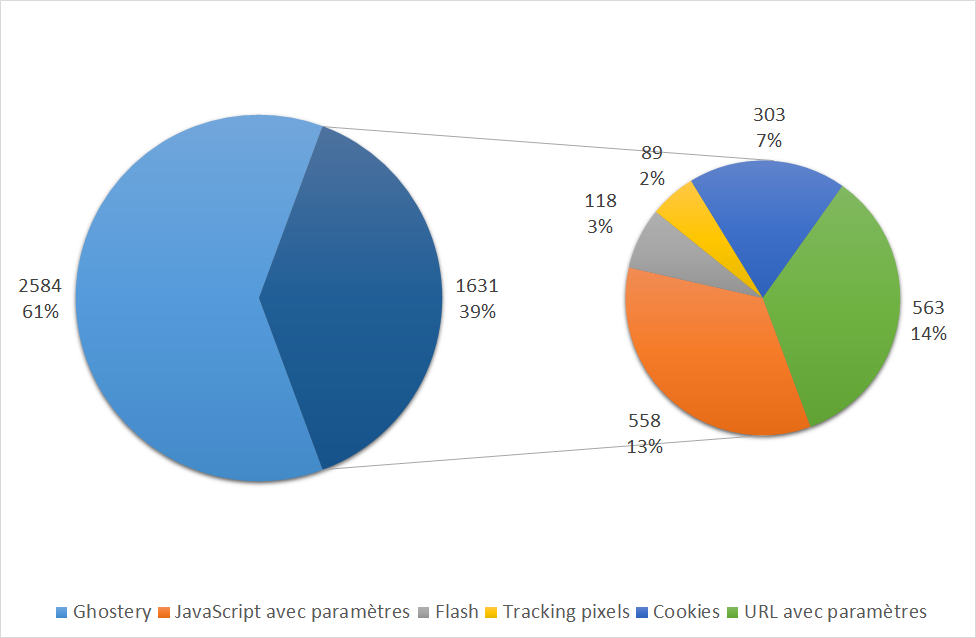
\includegraphics[scale=.6]{resultats/ANALYSES/Images/AdblockDefault-Ghostery.png}
	\caption{\label{exp-AdblockDefault-ghostery}Répartition des trackers par catégorie.}
\end{figure}

L'extension a laissé passer 2584 trackers connus de la base de données Ghostery et 1631 éléments ont été identifiés comme trackers selon les critères de l'outil.\\

\begin{tabular}{ c | p{5cm} | c | c || c | }
   Rang & Répartition des trackers & \# & \% & Evolution \\
   \hline
   \hline
   1 & Ghostery & 2584 & 61,30 & - 89,51\% \\
   2 & URL avec paramètres & 563 & 13,36 & - 58,30\% \\
   3 & JavaScript avec paramètres & 558 & 13,24 & - 48,29\% \\
   4 & Cookies & 303 & 7,19 & - 65,88\% \\
   5 & Flash & 118 & 2,80 & - 52,03\% \\
   6 & Tracking pixels & 89 & 2,11 & - 92,66\% \\
   \hline
    & TOTAL & 4215 & - & - 85,66\%\\
   \hline
\end{tabular}
\\[1cm]

\begin{tabular}{ c | p{5cm} | c | c | c | }
   Rang & Types MIME (Ghostery) & \# & \% & Evolution\\
   \hline
   \hline
   1 & JavaScript & 1136 & 43,96 & - 83,68\% \\
   2 & Images .png & 396 & 15,33 & - 59,09\% \\
   3 & HTML & 322 & 12,46 & - 93,33\% \\
   4 & Images .jpeg & 300 & 11,61 & - 56,08\% \\
   5 & Images .gif & 151 & 5,84 & -97,97\% \\
   \hline
\end{tabular}
\\[.3cm]

Deux baisses flagrantes sont constatées pour les pixels de traçage et les trackers connus de Ghostery. Dans ces derniers, ce sont principalement les images .gif, les requêtes de ressources HTML et les JavaScript qui sont bloqués par Adblock.

%Concernant les trackers bloqués par la base de données Ghostery, 1136 sont du JavaScript (en rassemblant les types \textit{application/x-javascript} (645), \textit{application/javascript} (264) et \textit{text/javascript} (227)). La deuxième position est occupée par les images \textit{.png} (396) et le trio de tête termine avec les images \textit{.jpeg} (300). Les trackers sous la forme d'images {.gif} semblent avoir bien été bloqués car ils ne sont que 151. Notons également la présence de 149 éléments de type {.css} jouant le rôle de trackers.

%Les 1631 autres éléments (graphique en secteurs visible à droite) sont constitués essentiellement d'URL avec une chaîne de requête (563 éléments, 14\%), de 558 codes JavaScript avec paramètres (13\%) et de réponses créant un cookie tiers (303, 7\%). Peu de pixels de traçage ont été détectés car ils ne sont qu'au nombre de 89 (2\%). Par contre, 118 ressources Flash ont été chargées depuis un domaine externe (3\%).

\subsubsection{Résultats de la seconde expérience - \autoref{exp-AdblockNoAcceptableAds-ghostery}}
\begin{figure}[!h]
	\centering
	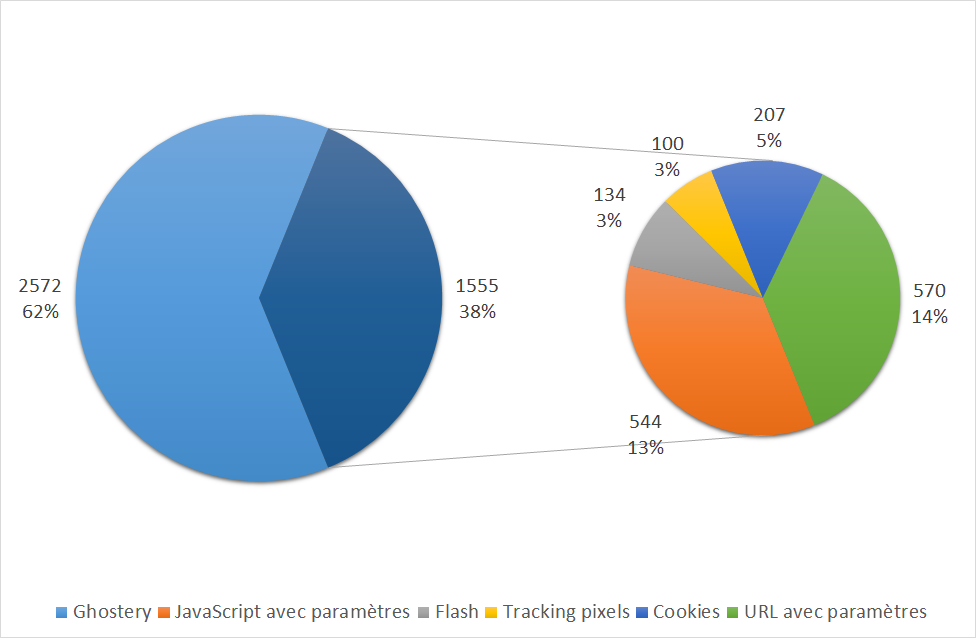
\includegraphics[scale=.6]{resultats/ANALYSES/Images/AdblockNoAcceptableAds-Ghostery.png}
	\caption{\label{exp-AdblockNoAcceptableAds-ghostery}Répartition des trackers par catégorie.}
\end{figure}

L'extension a laissé passer 2572 trackers connus de la base de données Ghostery et 1555 éléments ont été identifiés comme trackers selon les critères de l'outil.\\

\begin{tabular}{ c | p{5cm} | c | c || c | }
   Rang & Répartition des trackers & \# & \% & Evolution \\
   \hline
   \hline
   1 & Ghostery & 2572 & 62,32 & - 89,56\% \\
   2 & URL avec paramètres & 570 & 13,81 & - 57,78\% \\
   3 & JavaScript avec paramètres & 544 & 13,18 & - 49,58\% \\
   4 & Cookies & 207 & 5,02 & - 76,69\% \\
   5 & Flash & 134 & 3,25 & - 45,53\% \\
   6 & Tracking pixels & 100 & 2,42 & - 91,75\% \\
   \hline
    & TOTAL & 4127 & - & - 85,96\%\\
   \hline
\end{tabular}
\\[1cm]

\begin{tabular}{ c | p{5cm} | c | c | c | }
   Rang & Types MIME (Ghostery) & \# & \% & Evolution\\
   \hline
   \hline
   1 & JavaScript & 1134 & 44,09 & - 83,70\% \\
   2 & Images .png & 407 & 15,82 & - 57,95\% \\
   4 & HTML & 330 & 12,83 & - 93,17\% \\
   4 & Images .jpeg & 245 & 9,53 & - 64,13\% \\
   5 & Images .gif & 161 & 6,26 & - 97,84\% \\
   \hline
\end{tabular}
\\[.3cm]

Le fait de bloquer les publicités dites acceptables par les développeurs d'Adblock fait baisser un peu plus le niveau de trackers détectés : on passe de 4215 à 4127 trackers. Cette baisse est essentiellement causée par la diminution du nombre de réponses HTTP créant un cookie tiers (on diminue de 300 à 207). On constate également un nombre légèrement supérieur pour les ressources Flash, les pixels de traçage et les URL avec paramètres. Après vérification du log du \textit{parser}, 4 fichiers HTTP Archive ont été analysés en plus, ce qui provoque probablement ces légères hausses.

\subsubsection{Résultats de la troisième expérience - \autoref{exp-AdblockFanboyUltimate-ghostery}}
\begin{figure}[!h]
	\centering
	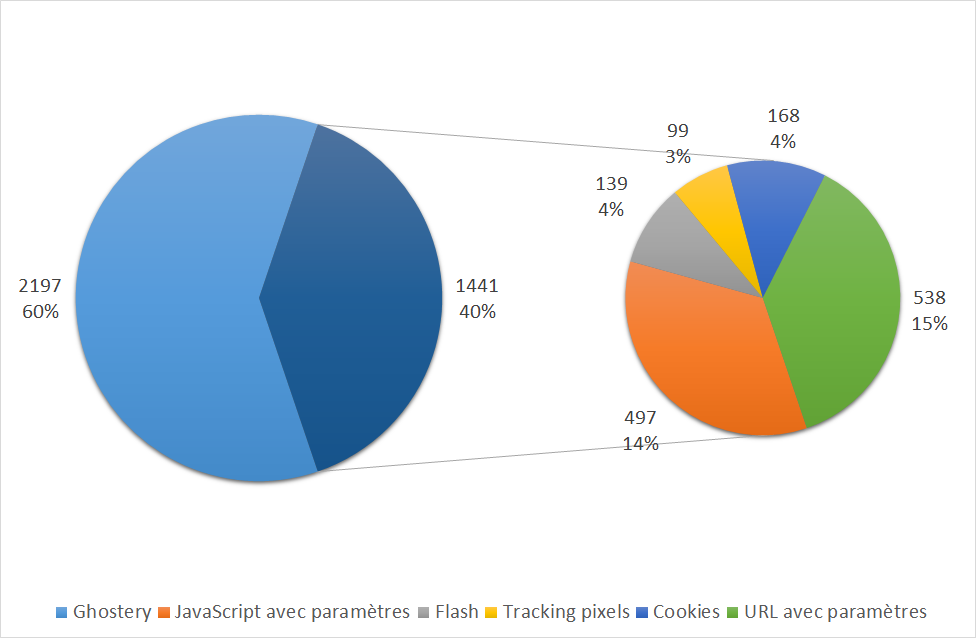
\includegraphics[scale=.6]{resultats/ANALYSES/Images/AdblockFanboyUltimate-Ghostery.png}
	\caption{\label{exp-AdblockFanboyUltimate-ghostery}Répartition des trackers par catégorie.}
\end{figure}

L'extension a laissé passer 2197 trackers connus de la base de données Ghostery et 1441 éléments ont été identifiés comme trackers selon les critères de l'outil.\\

\begin{tabular}{ c | p{5cm} | c | c || c | }
   Rang & Répartition des trackers & \# & \% & Evolution \\
   \hline
   \hline
   1 & Ghostery & 2197 & 60,39 & - 91,08\% \\
   2 & URL avec paramètres & 538 & 14,79 & - 60,15\% \\
   3 & JavaScript avec paramètres & 497 & 13,66 & - 53,94\% \\
   4 & Cookies & 168 & 4,62 & - 81,08\% \\
   5 & Flash & 139 & 3,82 & - 43,50\% \\
   6 & Tracking pixels & 99 & 2,72 & - 91,83\% \\
   \hline
    & TOTAL & 3638 & - & - 87,63\%\\
   \hline
\end{tabular}
\\[1cm]

\begin{tabular}{ c | p{5cm} | c | c | c | }
   Rang & Types MIME (Ghostery) & \# & \% & Evolution\\
   \hline
   \hline
   1 & JavaScript & 764 & 34,77 & - 89,02\% \\
   2 & Images .png & 373 & 16,98 & - 61,47\% \\
   3 & HTML & 318 & 14,47 & - 93,42\% \\
   4 & Images .jpeg & 316 & 14,38 & - 53,73\% \\
   5 & Images .gif & 152 & 6,92 & - 97,96\% \\
   \hline
\end{tabular}
\\[.3cm]

L'utilisation de la liste Fanboy Ultimate fait baisser davantage le nombre de trackers car on passe de 4127 pour l'expérience précédente (4215 pour la configuration par défaut d'Adblock) à 3638 trackers détectés. Pour les trackers de la base de données Ghostery, la baisse vient principalement du JavaScript avec une baisse de 1134 (1136 pour la configuration par défaut d'Adblock) à 764 codes JavaScript connus comme trackers ayant été détectés. Concernant les autres critères, une légère baisse des URL et JavaScript avec des paramètres est visible ainsi que pour les cookies.

%%%%%%%%%%
\subsection{DoNotTrackMe}
\subsubsection{Présentation}
DoNotTrackMe \footnote{\url{https://www.abine.com/donottrackme.html}} est une extension disponible pour Google Chrome, Firefox, Safari, Opera et Internet Explorer.
Elle bloque les trackers de différents types de sociétés (régies publicitaires, réseaux sociaux et sociétés qui récupèrent des données sur la navigation des utilisateurs). Il est expliqué sur le site de l'extension que son but n'est pas de bloquer toutes les publicités mais plutôt de bloquer les publicités ciblées qui utilisent des informations personnelles. Son fonctionnement repose sur une base de données de trackers. A chaque page ouverte dans le navigateur, l'extension vérifie les ressources qui sont chargées et bloque celles qui sont connues comme trackers.

\subsubsection{Configuration de l'extension}
L'extension n'a pas été configurée, les paramètres par défaut ont été laissés d'application. A vrai dire, les options de configuration sont assez rudimentaires. L'extension possède un écran de contrôle qui compte le nombre de trackers bloqués. Un compte premium est également proposé mais il n'est pas intéressant vu les fonctionnalités recherchées au sein de l'expérience.

\subsubsection{Résultats - \autoref{exp-DoNotTrackMe-ghostery}}
\begin{figure}[!h]
	\centering
	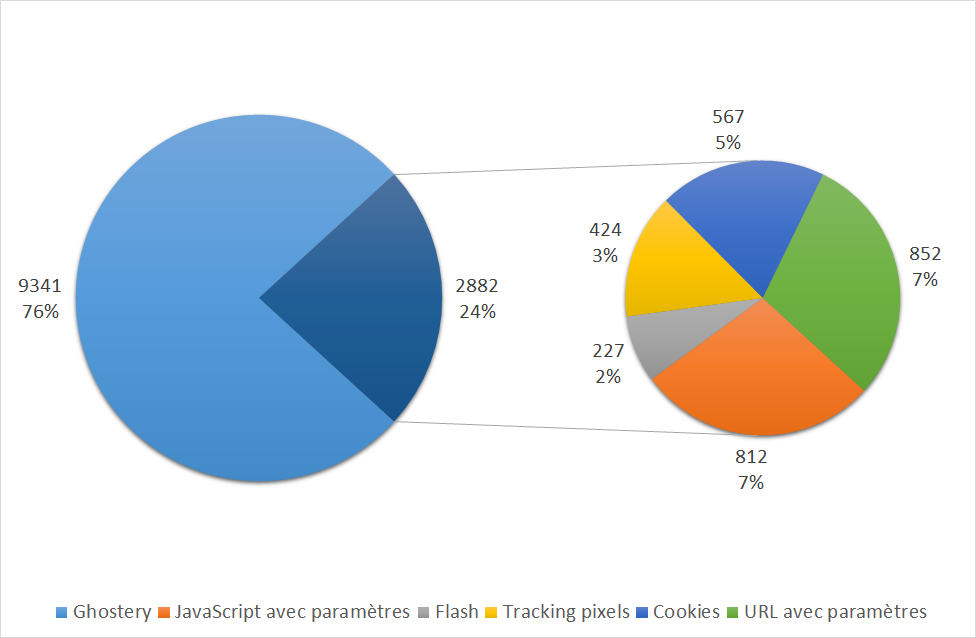
\includegraphics[scale=.6]{resultats/ANALYSES/Images/DoNotTrackMe-Ghostery.png}
	\caption{\label{exp-DoNotTrackMe-ghostery}Répartition des trackers par catégorie.}
\end{figure}

L'extension a laissé passer 9341 trackers connus de la base de données Ghostery et 2882 éléments ont été identifiés comme trackers selon les critères de l'outil.\\

\begin{tabular}{ c | p{5cm} | c | c || c | }
   Rang & Répartition des trackers & \# & \% & Evolution \\
   \hline
   \hline
   1 & Ghostery & 9341 & 76,42 & - 62,07\% \\
   2 & URL avec paramètres & 852 & 6,97 & - 36,89\% \\
   3 & JavaScript avec paramètres & 812 & 6,64 & - 24,75\% \\
   4 & Cookies & 567 & 4,64 & - 36,15\% \\
   5 & Tracking pixels & 424 & 3,47 & - 65,02\% \\
   6 & Flash & 227 & 1,86 & - 7,72\% \\
   \hline
    & TOTAL & 12223 & - & - 58,43\%\\
   \hline
\end{tabular}
\\[1cm]

\begin{tabular}{ c | p{5cm} | c | c | c | }
   Rang & Types MIME (Ghostery) & \# & \% & Evolution\\
   \hline
   \hline
   1 & JavaScript & 3441 & 36,84 & - 50,55\% \\
   2 & Images .gif & 2124 & 22,74 & - 71,51\% \\
   3 & HTML & 1400 & 14,99 & - 71,01\% \\
   4 & Type inconnu & 529 & 5,66 & - 67,82\% \\
   5 & Images .png & 517 & 5,53 & - 46,59\% \\
   \hline
\end{tabular}
\\[.3cm]

L'extension offre une protection relativement moyenne car elle ne bloque que 58,43\% des trackers par rapport à l'expérience de référence. Elle bloque cependant 65,02\% de pixels de traçage et 62,07\% des trackers connus par Ghostery. Dans ces derniers, ce sont les pixels de traçage (71,51\%) et les URL avec une chaîne de requête qui sont proportionnellement les plus bloqués (71,01\% pour le type HTML et 67,82\% pour les types inconnus). Quant aux codes JavaScript, ils sont en tête avec 3441 trackers bloqués.

%%%%%%%%%%
\subsection{Ghostery}
\subsubsection{Présentation}
Ghostery \footnote{\url{https://www.ghostery.com}} est une extension disponible pour Firefox, Google Chrome, Opera et Safari. Son fonctionnement repose sur une base de données de trackers alimentée par les retours des utilisateurs de l'extension. Cette base de données est régulièrement mise à jour. Evidon, la société qui possède Ghostery, a fait momentanément parler d'elle car elle a des contrats avec certaines entreprises. Certains lui reprochaient alors de vendre les informations reçues des utilisateurs via son programme Ghostrank. Sur leur site, les développeurs de Ghostery assurent ne pas vendre d'informations personnelles. Il faut noter qu'il est possible d'utiliser Ghostery sans activer Ghostrank.

\subsubsection{Configuration de l'extension}
L'extension a été activée avec tous les trackers et tous les cookies sélectionnés.

\subsubsection{Résultats - \autoref{exp-Ghostery-ghostery}}
\begin{figure}[!h]
	\centering
	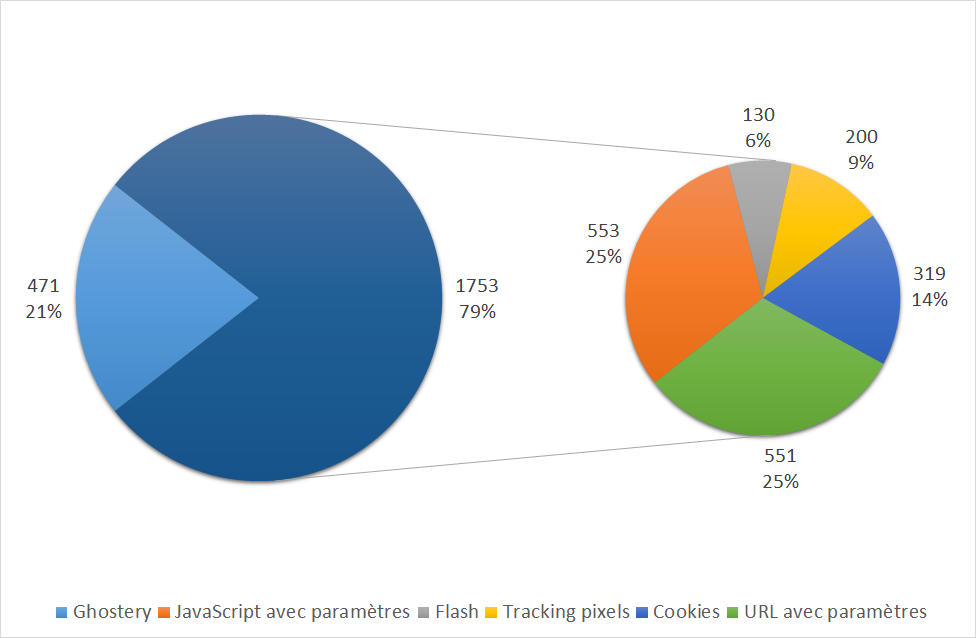
\includegraphics[scale=.6]{resultats/ANALYSES/Images/Ghostery-Ghostery.png}
	\caption{\label{exp-Ghostery-ghostery}Répartition des trackers par catégorie.}
\end{figure}

L'extension a laissé passer 471 trackers connus de la base de données Ghostery et 1753 éléments ont été identifiés comme trackers selon les critères de l'outil.\\

\begin{tabular}{ c | p{5cm} | c | c || c | }
   Rang & Répartition des trackers & \# & \% & Evolution \\
   \hline
   \hline
   1 & JavaScript avec paramètres & 553 & 14,53 & - 48,75\% \\
   2 & URL avec paramètres & 551 & 14,48 & - 59,19\% \\
   3 & Ghostery & 471 & 12,38 & - 98,09\% \\
   4 & Cookies & 319 & 8,38 & - 64,08\% \\
   5 & Tracking pixels & 200 & 5,25 & - 83,50\% \\
   6 & Flash & 130 & 3,42 & - 47,15\% \\
   \hline
    & TOTAL & 2224 & - & - 92,44\%\\
   \hline
\end{tabular}
\\[1cm]

\begin{tabular}{ c | p{5cm} | c | c | c | }
   Rang & Types MIME (Ghostery) & \# & \% & Evolution\\
   \hline
   \hline
   1 & Images .png & 111 & 23,57 & - 88,53\% \\
   2 & Images .jpeg & 92 & 19,53 & - 86,53\% \\
   3 & JavaScript & 86 & 18,26 & - 98,76\% \\
   4 & Images .gif & 62 & 13,16 & - 99,17\% \\
   5 & HTML & 56 & 11,89 & - 98,84\% \\
   \hline
\end{tabular}
\\[.3cm]

Les résultats de l'analyse ont été assez étonnants car ils montrent qu'une partie des trackers n'est pas bloquée par Ghostery alors qu'ils sont bien présents dans la base de données. Ils sont détectés par le \textit{parser} qui utilise la même base de données. Une analyse plus poussée sur les liens non bloqués a été effectuée. Le constat était que Ghostery ne bloque pas les trackers du site visité (les trackers "first-party"). Après une recherche, la justification a été trouvé sur un billet de blog \footnote{\url{https://purplebox.ghostery.com/post/1016021484}} des développeurs de l'extension. La raison principale est que bloquer ces trackers peut entraîner des interférences lors de l'utilisation des fonctionnalités du site.

Néanmoins, l'extension offre une bonne protection car elle bloque 92,44\% des trackers. Les principaux trackers non bloqués sur les sites visités sont les images .png et .jpeg (respectivement 23,57\% et 19,53\%), suivies des JavaScript (18,26\%) et des images .gif (13,16\%).
Concernant les autres critères, les pixels de traçage sont relativement bien bloqués avec un taux de 83,50\%, cela signifie que 200 pixels passent quand même à côté de la base de données Ghostery.

%%%%%%%%%%
\subsection{HTTPS Everywhere}
\subsubsection{Présentation}
HTTPS Everywhere \footnote{\url{https://www.eff.org/https-everywhere}} est une extension disponible pour Firefox, Google Chrome, Opera et Android. Firefox dispose d'une version stable tandis que les autres n'ont accès qu'à une version beta. Le but de cette extension est d'utiliser les connexions HTTPS dès que cela est possible. L'extension repose sur une liste afin de savoir quand passer d'une connexion HTTP vers une connection HTTPS. Par défaut, l'extension contient une liste de règles prédéfinies pour chaque site mais il est également possible de créer ses propres règles.
Grâce à l'utilisation de connections sécurisées, l'extension protège l'utilisateur de certaines attaques. Dès qu'une connection sécurisée peut être établie vers un site, HTTPS Everywhere le fait. Il peut cependant arriver que certaines requêtes vers un site soient en HTTP alors que d'autres sont en HTTPS. L'extension n'est pas en mesure de protéger l'utilisateur si le site ne propose pas de connection HTTPS pour toutes ses ressources.

\subsubsection{Configuration de l'extension}
L'extension a été installée avec ses paramètres par défaut. SSL Observatory n'a pas été activé et aucune règle supplémentaire n'a été ajoutée.

\subsubsection{Résultats - \autoref{exp-HTTPSEverywhere-ghostery}}
\begin{figure}[!h]
	\centering
	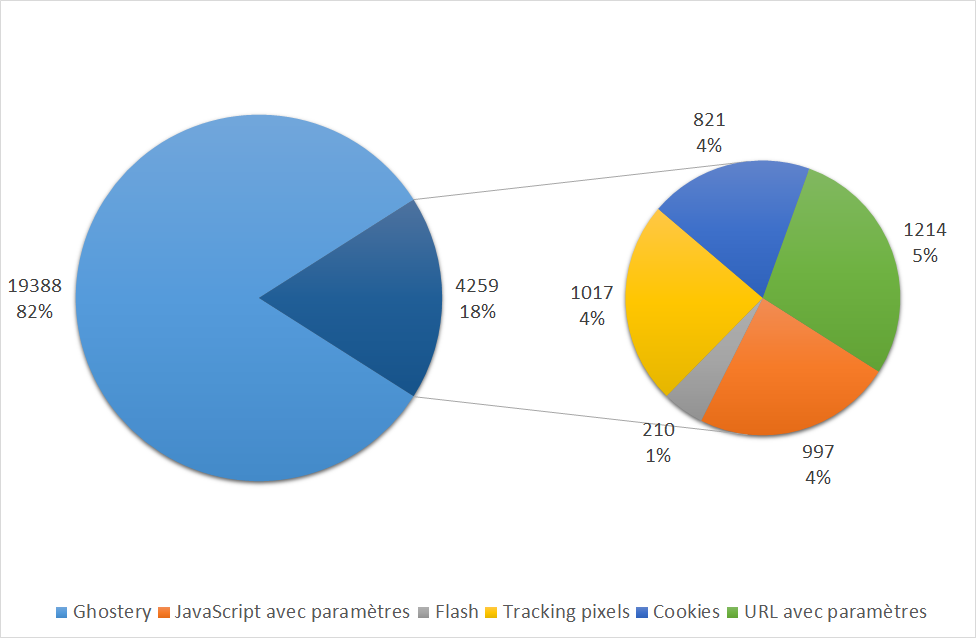
\includegraphics[scale=.6]{resultats/ANALYSES/Images/HTTPSEverywhere-Ghostery.png}
	\caption{\label{exp-HTTPSEverywhere-ghostery}Répartition des trackers par catégorie.}
\end{figure}

L'extension a laissé passer 19388 trackers connus de la base de données Ghostery et 4259 éléments ont été identifiés comme trackers selon les critères de l'outil.\\

\begin{tabular}{ c | p{5cm} | c | c || c | }
   Rang & Répartition des trackers & \# & \% & Evolution \\
   \hline
   \hline
   1 & Ghostery & 19388 & 81,99 & - 21,27\% \\
   2 & URL avec paramètres & 1214 & 5,13 & - 10,07\% \\
   3 & Tracking pixels & 1017 & 4,30 & - 16,09\% \\
   4 & JavaScript avec paramètres & 997 & 4,22 & - 7,60\% \\
   5 & Cookies & 821 & 3,47 & - 7,55\% \\
   6 & Flash & 210 & 0,89 & - 14,63\% \\
   \hline
    & TOTAL & 23647 & - & - 19,57\%\\
   \hline
\end{tabular}
\\[1cm]

\begin{tabular}{ c | p{5cm} | c | c | c | }
   Rang & Types MIME (Ghostery) & \# & \% & Evolution\\
   \hline
   \hline
   1 & Images .gif & 5817 & 30,00 & - 21,98\% \\
   2 & JavaScript & 5659 & 29,19 & - 18,68\% \\
   3 & HTML & 3782 & 19,51 & - 21,70\% \\
   4 & Type inconnu & 1142 & 5,89 & - 30,54\% \\
   5 & Texte & 826 & 4,26 & - 22,73\% \\
   \hline
\end{tabular}
\\[.3cm]

HTTPS Everywhere n'est pas une extension dont le but est de protéger la vie privée mais la motivation pour cette expérience était de voir si le fait de se connecter en HTTPS à des sites avait une incidence sur le nombre de trackers. D'après les résultats, il semble que oui car on observe une baisse de 19,57\% du nombre de trackers par rapport à la référence.


%%%%%%%%%%
\subsection{Priv3}
\subsubsection{Présentation}
Priv3 \footnote{\url{http://priv3.icsi.berkeley.edu/}} est une extension uniquement disponible pour Firefox. Son but est de bloquer le tracking effectué par les réseaux sociaux. Priv3 ne bloque pas complètement toutes les interactions tierces, elle supprime de manière sélective l'inclusion de cookies tiers quand le navigateur récupère du contenu provenant des réseaux sociaux mais les réactive lorsqu'on veut interagir avec les modules des réseaux sociaux.
\newline

L'extension gère les réseaux sociaux suivants: Facebook, Twitter, Google+ et LinkedIn. Cependant, elle ne semble plus mise à jour depuis juillet 2011.

\subsubsection{Configuration de l'extension}
Aucun paramètre de configuration n'est disponible pour cette extension.

\subsubsection{Résultats - \autoref{exp-Priv3-ghostery}}
\begin{figure}[!h]
	\centering
	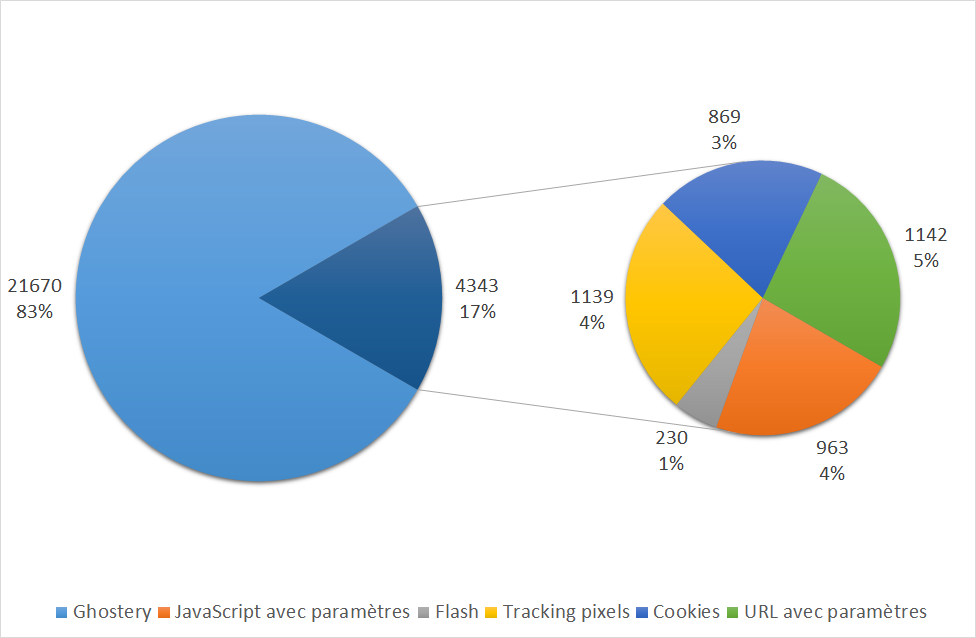
\includegraphics[scale=.6]{resultats/ANALYSES/Images/Priv3-Ghostery.png}
	\caption{\label{exp-Priv3-ghostery}Répartition des trackers par catégorie.}
\end{figure}

L'extension a laissé passer 21670 trackers connus de la base de données Ghostery et 4343 éléments ont été identifiés comme trackers selon les critères de l'outil.\\

\begin{tabular}{ c | p{5cm} | c | c || c | }
   Rang & Répartition des trackers & \# & \% & Evolution \\
   \hline
   \hline
   1 & Ghostery & 21670 & 83,30 & - 12,01\% \\
   2 & URL avec paramètres & 1142 & 4,39 & - 15,41\% \\
   3 & Tracking pixels & 1139 & 4,38 & - 6,02\% \\
   4 & JavaScript avec paramètres & 963 & 3,70 & - 10,75\% \\
   5 & Cookies & 869 & 3,34 & - 2,14\% \\
   6 & Flash & 230 & 0,88 & - 6,50\% \\
   \hline
    & TOTAL & 26013 & - & - 11,53\%\\
   \hline
\end{tabular}
\\[1cm]

\begin{tabular}{ c | p{5cm} | c | c | c | }
   Rang & Types MIME (Ghostery) & \# & \% & Evolution\\
   \hline
   \hline
   1 & JavaScript & 6484 & 29,92 & - 6,83\% \\
   2 & Images .gif & 6137 & 28,32 & - 17,69\% \\
   3 & HTML & 4307 & 19,88 & - 10,83\% \\
   4 & Type inconnu & 1418 & 6,54 & - 13,75\% \\
   5 & Texte & 954 & 4,40 & - 10,76\% \\
   \hline
\end{tabular}
\\[.3cm]

Priv3 a pour objectif de bloquer les trackers de 4 plateformes de réseaux sociaux. Le but de cette expérience n'était donc pas de voir si l'extension bloquait un nombre important de trackers mais plutôt d'estimer la proportion que représentent les réseaux sociaux dans les trackers. L'extension a bloqué 11,53\% de trackers dont 12,01\% de trackers connus dans la base de données Ghostery. Parmi ces derniers, les images .gif sont proportionnellement les plus bloquées avec une baisse de 17,69\% mais ce sont les JavaScript qui sont en tête avec 6484 trackers de ce type ayant été détectés.


%%%%%%%%%%
\subsection{Privacy Badger}
\subsubsection{Présentation}
Privacy Badger \footnote{\url{https://www.eff.org/privacybadger}} est une extension disponible pour Firefox et Google Chrome, elle est actuellement en version alpha. Son but est de bloquer les trackers de domaines tiers grâce à l'analyse de leur comportement. 
Lors de l'envoi d'une requête, un entête Do Not Track est ajouté et l'extension évalue la probabilité d'être tracké grâce à des heuristiques. L'extension enregistre diverses informations afin d'affiner son fonctionnement en fonction des sites visités. Il faut donc un certain temps pour que l'utilisateur soit mieux protégé.

L'extension contient aussi une liste blanche pour certains domaines qui fournissent des ressources tierces essentielles. A long terme, les développeurs espèrent se séparer de cette liste grâce aux promesses des domaines tiers de respecter Do Not Track. Le but de Privacy Badger n'est pas de bloquer les publicités mais de prévenir les invasions indésirables dans la vie privée des utilisateurs. 
Actuellement, seul le tracking provenant de tiers est bloqué. Dans le futur, les développeurs comptent également ajouter des protections pour les sites visités et ils vont ajouter des contre-mesures pour bloquer les fingerprinters dans une prochaine version.

\subsubsection{Configuration de l'extension}
L'extension est restée configurée avec les paramètres par défaut.

\subsubsection{Résultats - \autoref{exp-PrivacyBadger-ghostery}}
\begin{figure}[!h]
	\centering
	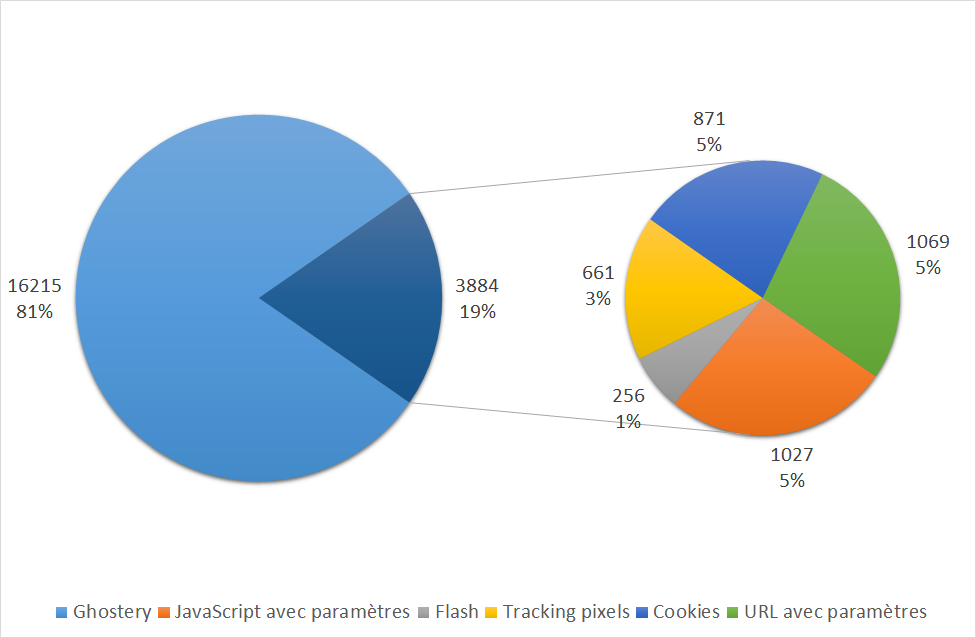
\includegraphics[scale=.6]{resultats/ANALYSES/Images/PrivacyBadger-Ghostery.png}
	\caption{\label{exp-PrivacyBadger-ghostery}Répartition des trackers par catégorie.}
\end{figure}

L'extension a laissé passer 16215 trackers connus de la base de données Ghostery et 3884 éléments ont été identifiés comme trackers selon les critères de l'outil.\\

\begin{tabular}{ c | p{5cm} | c | c || c | }
   Rang & Répartition des trackers & \# & \% & Evolution \\
   \hline
   \hline
   1 & Ghostery & 16215 & 80,68 & - 34,16\% \\
   2 & URL avec paramètres & 1069 & 5,32 & - 20,81\% \\
   3 & JavaScript avec paramètres & 1027 & 5,11 & - 4,82\% \\
   4 & Cookies & 871 & 4,33 & - 1,91\% \\
   5 & Tracking pixels & 661 & 3,29 & - 45,46\% \\
   6 & Flash & 256 & 1,27 & + 4,07\% \\
   \hline
    & TOTAL & 20099 & - & - 31,64\%\\
   \hline
\end{tabular}
\\[1cm]

\begin{tabular}{ c | p{5cm} | c | c | c | }
   Rang & Types MIME (Ghostery) & \# & \% & Evolution\\
   \hline
   \hline
   1 & JavaScript & 5490 & 33,86 & - 21,11\% \\
   2 & Images .gif & 4716 & 29,08 & - 36,75\% \\
   3 & HTML & 2851 & 17,58 & - 40,97\% \\
   4 & Type inconnu & 900 & 5,55 & - 45,26\% \\
   5 & Texte & 601 & 3,71 & - 43,78\% \\
   \hline
\end{tabular}
\\[.3cm]

L'extension bloque un peu moins d'un tiers des trackers. Les trackers connus de Ghostery sont en tête des trackers bloqués avec un nombre de 16215 mais ils ne représentent qu'une baisse de 34,16\% alors que les pixels de traçage sont mieux bloqués avec une baisse de 45,46\%. Le taux de détection de fichiers Flash est en hausse, cela s'explique par un nombre plus important de fichiers analysés (9 fichiers supplémentaires) par le \textit{parser}.


%%%%%%%%%%
\subsection{Adblock \& Ghostery}
\subsubsection{Configuration des extensions}

\subsubsection{Résultats - \autoref{exp-AdblockGhostery-ghostery}}
\begin{figure}[!h]
	\centering
	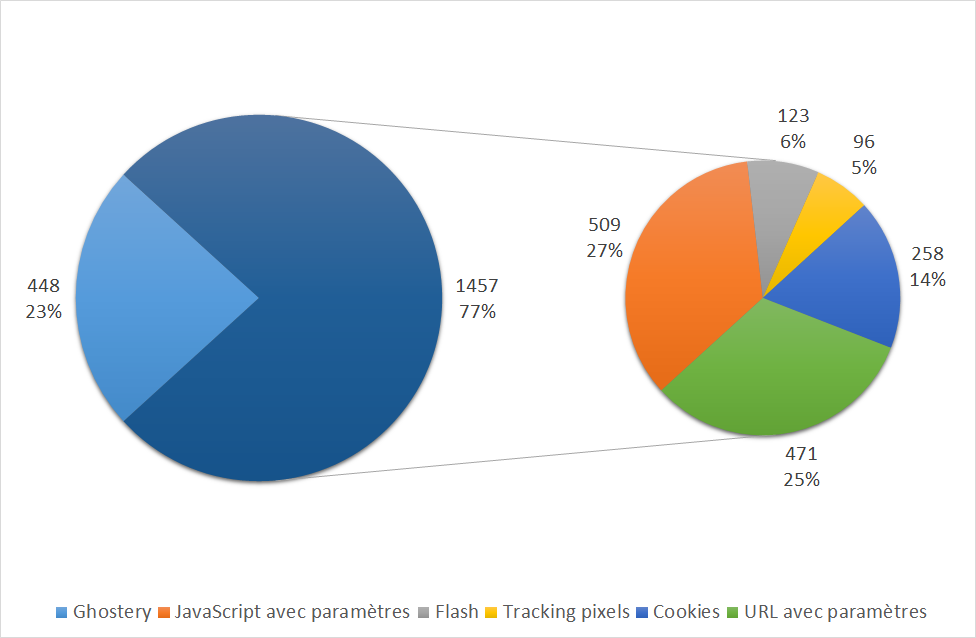
\includegraphics[scale=.6]{resultats/ANALYSES/Images/AdblockGhostery-Ghostery.png}
	\caption{\label{exp-AdblockGhostery-ghostery}Répartition des trackers par catégorie.}
\end{figure}

Les extensions ont laissé passer 448 trackers connus de la base de données Ghostery et 1457 éléments ont été identifiés comme trackers selon les critères de l'outil.\\

\begin{tabular}{ c | p{5cm} | c | c || c | }
   Rang & Répartition des trackers & \# & \% & Evolution \\
   \hline
   \hline
   1 & JavaScript avec paramètres & 509 & 26,72 & - 52,83\% \\
   2 & URL avec paramètres & 471 & 24,72 & - 65,11\% \\
   3 & Ghostery & 448 & 23,52 & - 98,18\% \\
   4 & Cookies & 258 & 13,54 & - 70,95\% \\
   5 & Flash & 123 & 6,46 & - 50,00\% \\
   6 & Tracking pixels & 96 & 5,04 & - 92,08\% \\
   \hline
    & TOTAL & 1905 & - & - 93,52\%\\
   \hline
\end{tabular}
\\[1cm]

\begin{tabular}{ c | p{5cm} | c | c | c | }
   Rang & Types MIME (Ghostery) & \# & \% & Evolution\\
   \hline
   \hline
   1 & Images .jpeg & 176 & 39,29 & - 74,23\% \\
   2 & Images .png & 100 & 22,32 & - 89,67\% \\
   3 & JavaScript & 63 & 14,06 & - 99,09\% \\
   4 & HTML & 39 & 8,71 & - 99,19\% \\
   5 & Images .gif & 31 & 6,92 & - 99,58\% \\
   \hline
\end{tabular}
\\[.3cm]

Cette expérience avait pour but de tester ensemble les deux extensions ayant les meilleurs résultats. Il en ressort que les extensions combinées apportent des résultats encore meilleurs car on atteint un taux de blocage de 93,52\%. Ceci s'explique par le fait qu'Adblock bloque plus de trackers non bloqués par Ghostery, notamment les pixels de traçage et les réponses HTTP qui créent un cookie tiers. D'un autre côté, Ghostery bloque des trackers qui ne sont pas présents dans les listes d'Adblock. Ces deux effets font que le nombre global de trackers diminue davantage afin d'atteindre le meilleur taux de protection.


\section{Do Not Track}
\subsection{Présentation}
Do Not Track \footnote{\url{http://donottrack.us/}} est un entête HTTP qui signale au serveur le souhait de l'utilisateur de ne pas être tracé. Les sites ont le choix d'accepter ce souhait ou de l'ignorer car il n'y a aucun effet contraignant s'ils ne le respectent pas.

L'activation se fait aisément dans les paramètres du navigateur, il ne s'agit que d'une simple case à cocher.

Le but de cette expérience était de voir si les sites respectent cet entête en regardant si le nombre de trackers détectés diminue de façon significative.

\subsection{Résultats - \autoref{exp-DNT-ghostery}}
\begin{figure}[!h]
	\centering
	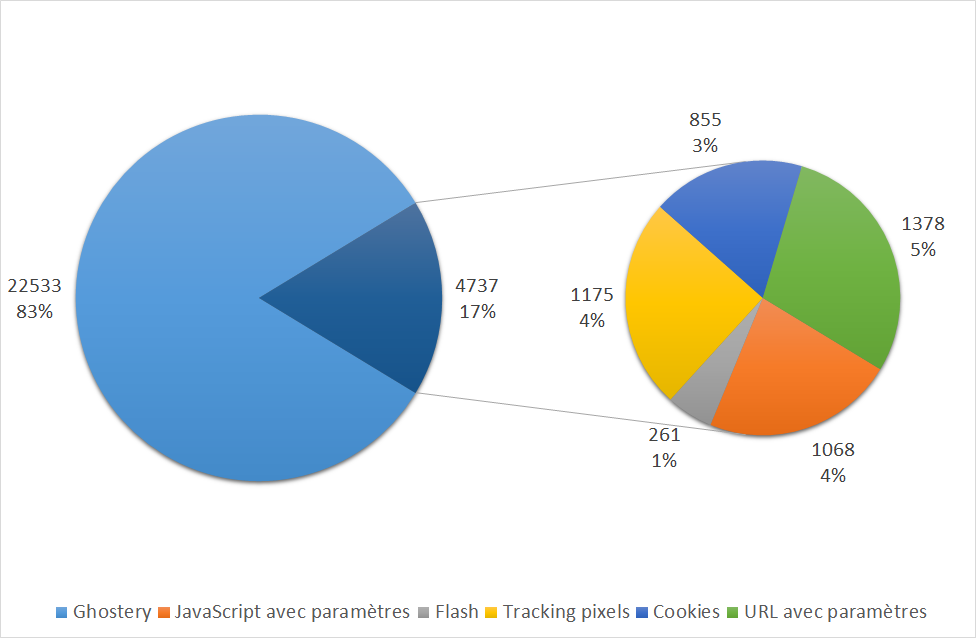
\includegraphics[scale=.6]{resultats/ANALYSES/Images/DNT-Ghostery.png}
	\caption{\label{exp-DNT-ghostery}Répartition des trackers par catégorie.}
\end{figure}

Do Not Track a laissé passer 22533 trackers connus de la base de données Ghostery et 4737 éléments ont été identifiés comme trackers selon les critères de l'outil.\\

\begin{tabular}{ c | p{5cm} | c | c || c | }
   Rang & Répartition des trackers & \# & \% & Evolution \\
   \hline
   \hline
   1 & Ghostery & 22533 & 82,63 & - 8,50\% \\
   2 & URL avec paramètres & 1378 & 5,05 & + 2,07\% \\
   3 & Tracking pixels & 1175 & 4,31 & - 3,05\% \\
   4 & JavaScript & 1068 & 3,92 & - 1,02\% \\
   5 & Cookies & 855 & 3,14 & - 3,72\% \\
   6 & Flash & 261 & 0,96 & + 6,10\% \\
   \hline
    & TOTAL & 27270 & - & - 7,25\%\\
   \hline
\end{tabular}
\\[1cm]

\begin{tabular}{ c | p{5cm} | c | c | c | }
   Rang & Types MIME (Ghostery) & \# & \% & Evolution\\
   \hline
   \hline
   1 & Images .gif & 6597 & 29,28 & - 11,52\% \\
   2 & JavaScript & 6584 & 29,22 & - 5,39\% \\
   3 & HTML & 4473 & 19,85 & - 7,39\% \\
   4 & Type inconnu & 1151 & 5,11 & - 29,99\% \\
   5 & Texte & 1006 & 4,46 & - 5,89\% \\
   \hline
\end{tabular}
\\[.3cm]

Certains sites semblent respecter ce souhait car le nombre total de trackers détectés est en baisse de 7,25\%. Comme pour les autres expériences, les pourcentages en hausse dans l'évolution par rapport aux chiffres de référence proviennent d'un nombre légèrement plus élevé de fichiers analysés.
Activer l'entête Do Not Track ne permet pas de se protéger de manière efficace contre les trackers mais il a l'avantage d'être très simple à activer. De plus, cela montre un signe encourageant de la part de certains sites qui commencent à prendre conscience que les utilisateurs désirent un meilleur respect de leur vie privée lorsqu'ils naviguent sur Internet.


\section{Autres extensions intéressantes}
D'autres extensions relatives à la protection de la vie privée sont intéressantes mais n'avaient pas de raisons d'être testées avec l'outil. Elles sont néanmoins présentées dans cette section à titre d'information.

\subsection{BetterPrivacy}
BetterPrivacy \footnote{\url{https://addons.mozilla.org/fr/firefox/addon/betterprivacy/}} est une extension qui a pour but de supprimer les cookies Flash après chaque session de navigation. La raison pour laquelle elle n'a pas été testée est que le \textit{crawler} effectue l'ensemble des visites de sites au sein d'une même session. L'extension n'aurait donc pas pu être testé dans les conditions optimales d'utilisation.

\subsection{NoScript}
NoScript \footnote{\url{http://noscript.net/}} est une extension disponible pour Firefox qui a pour but de n'autoriser l'exécution que des scripts provenant de sites de confiance. Le test de cette extension n'aurait pas eu beaucoup de valeurs car il elle aurait bloqué l'ensemble des scripts, ce qui n'aurait pas été représentatif d'une utilisation normale d'Internet.

\section{Résultats}
\label{results_plugins}

\begin{figure}[!h]
	\hspace{-2cm}
	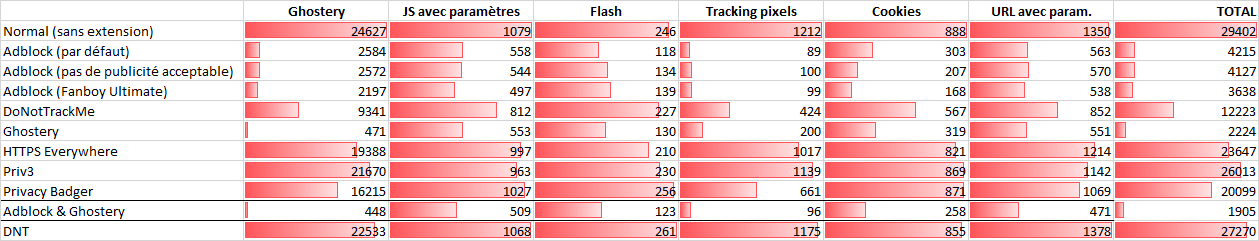
\includegraphics[scale=.54]{resultats/ANALYSES/Images/Comparaisons-Ghostery.png}
	\caption{\label{exp-DNT-ghostery}Comparaison des différents expériences (avec la base Ghostery).}
\end{figure}

\begin{figure}[!h]
	\hspace{-2cm}
	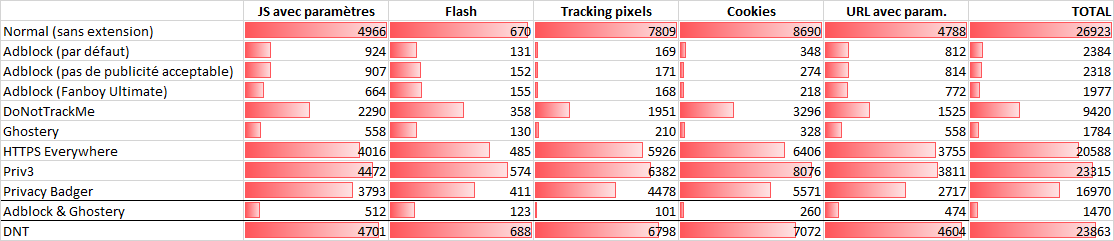
\includegraphics[scale=.6]{resultats/ANALYSES/Images/Comparaisons-NoG.png}
	\caption{\label{exp-DNT-ghostery}Comparaison des différents expériences (sans la base Ghostery).}
\end{figure}

Seule l'analyse utilisant la base de données Ghostery a été utilisée pour le calcul des résultats pour la raison évoquée dans la \autoref{extensions_navigateurs}. Cependant, ces deux tableaux permettent de constater que les deux types d'analyses fournissent proportionnellement les mêmes résultats sur les différentes expériences.
\newline

Ils permettent également de voir en un seul coup d'\oe{}il quelles sont les expériences qui donnent les meilleurs résultats.

La combinaison des extensions Adblock (avec la liste Fanboy Ultimate) et Ghostery offre la meilleure protection.

Si l'utilisateur ne désire installer qu'une seule extension, son choix devrait se porter sur Ghostery.
En effet, c'est l'extension qui obtient les meilleurs résultats même dans le type d'analyse qui n'utilise pas leur base de données. Elle est suivie par Adblock (équipée de la liste Fanboy Ultimate).



\chapter{Conclusion}

\appendix
\chapter{Options de l'outil implémenté}
\label{options_outil_implémenté}
Lors du lancement du \textit{crawler}, l'utilisateur peut spécifier plusieurs arguments :
\begin{itemize}
	\item Requis : le mode (\textit{crawler} ou \textit{parser}).
	\item Requis : le répertoire des fichiers.\\
		Pour le \textit{crawler}, il s'agit du répertoire où les fichiers seront enregistrés.\\
		Pour le \textit{parser}, il s'agit du répertoire contenant les fichiers à analyser.
	\item Optionnel : l'activation du mode \textit{debug} qui va donner davantage de détails en cas de problème.
	\item Optionnel : l'affichage de l'aide.
	\newline
	\item Requis pour le \textit{crawler} : le profil de Firefox à utiliser.
	\item Requis pour le \textit{crawler} : le fichier contenant la liste des sites web à visiter.
	\item Requis pour le \textit{crawler} : le début de l'intervalle des sites à visiter.
	\item Requis pour le \textit{crawler} : la fin de l'intervalle des sites à visiter.
	\item Requis pour le \textit{crawler} : le nombre maximal de tentatives par site web (\textit{timeout}).
	\item Requis pour le \textit{crawler} : le nombre de sites à visiter avant le redémarrage de Firefox.
	\newline
	\item Requis pour le \textit{parser} : le fichier contenant la liste des trackers de Ghostery.
	\item Optionnel pour le \textit{parser} : l'activation de l'impression de tous les trackers identifiés.
\end{itemize}

\chapter{Modifications dans l'extension NetExport}
\section{harBuilder.js}
\label{harBuilder}
Lignes 200 à 211 commentées :
\begin{lstlisting}[frame=single]
/*if (!timings._timeStamps)
{
  timings.comment = "_timeStamps field contains timing data generated using " + "console.timeStamp() method. See Firebug documentation: " + "http://getfirebug.com/wiki/index.php/Console_API";
  timings._timeStamps = [];
}

timings._timeStamps.push({
  time: stamp.time - this.startedDateTime,
  label: label
});*/
\end{lstlisting}

\section{automation.js}
\label{automation}
Ligne 171 modifiée :
\begin{lstlisting}[frame=single]
var fileName = name; /*+ "+" + now.getFullYear() + "-" + f(now.getMonth()+1) + "-" + f(now.getDate()) + "+" + f(now.getHours()) + "-" + f(now.getMinutes()) + "-" + f(now.getSeconds());*/
\end{lstlisting}


\chapter{Format des résultats}
\label{format_resultats}
Il existe deux types de résultats : les résultats détaillés pour chaque fichier HTTP Archive analysé et les résultats globaux de l'analyse.

Les résultats globaux sont enregistrés dans le dossier "logs" alors que les résultats détaillés sont enregistrés dans le dossier "results".
Ceci a été décidé par souci de simplicité car les résultats globaux sont ainsi directement accessibles et ne sont pas noyés dans le dossier contenant les résultats détaillés.

\section{Crawler}
Les résultats globaux dans le dossier "logs" :
\begin{itemize}
	\item \textbf{stats\_flash-cookies.csv} contient la liste des sites utilisant des cookies Flash, triés par ordre décroissant.
	%\newline
\end{itemize}

\section{Parser}
Les résultats globaux dans le dossier "logs" :
\begin{itemize}
	\item \textbf{stats\_detailed.csv} contient la liste des sites avec le nombre détaillé d'éléments enregistrés (trackers connus identifiés avec l'aide de Ghostery, réponses HTTP créant un cookie, fichiers JavaScript avec ou sans paramètres chargés depuis un autre domaine, Flash chargés depuis un autre domaine, pixels espions et requêtes d'URL avec des paramètres).
	\item \textbf{stats\_mimetypes\_ghostery.csv} contient la liste des types d'éléments (\textit{mimetype}) des trackers détectés par Ghostery, triés par ordre décroissant (si Ghostery a été utilisé par le \textit{parser}).
	\item \textbf{stats\_mimetypes\_soa.csv} contient la liste des types d'éléments (\textit{mimetype}) chargés d'un domaine différent, triés par ordre décroissant.
	\item \textbf{stats\_trackers.csv} contient la liste des trackers identifiés grâce à Ghostery, triés par ordre décroissant (si Ghostery a été utilisé par le \textit{parser}).
	\newline
\end{itemize}

Les résultats détaillés pour chaque site dans le dossier "results" :
\begin{itemize}
	\item \textbf{<URL du site>\_cookies.csv} contient la liste des cookies créés (avec leurs détails) par des réponses HTTP d'un domaine différent.
	\item \textbf{<URL du site>\_flash.csv} contient la liste des fichiers Flash provenant d'un autre domaine.
	\item \textbf{<URL du site>\_ghostery.csv} contient la liste des trackers détectés grâce à la base de données Ghostery (si Ghostery a été utilisé par le \textit{parser}).
	\item \textbf{<URL du site>\_js.csv} contient la liste des fichiers JavaScript provenant d'un domaine tiers.
	\item \textbf{<URL du site>\_js-query.csv} contient la liste des fichiers JavaScript provenant d'un domaine tiers et appelés avec des paramètres.
	\item \textbf{<URL du site>\_mimetypes.csv} contient la liste des types d'éléments (\textit{mimetype}) chargés d'un domaine différent, triés par ordre décroissant.
	\item \textbf{<URL du site>\_parameters.csv} contient la liste des requêtes vers un domaine différent dont l'URL contient des paramètres.
	\item \textbf{<URL du site>\_pixels.csv} contient la liste des pixels espions détectés depuis un autre domaine.
	\item \textbf{<URL du site>\_urls.csv} contient la liste de l'URL de toutes les ressources chargées d'un domaine différent.
	\newline
\end{itemize}


\bibliographystyle{unsrt}
\bibliography{bibliographie}

\end{document}
